\documentclass[12pt,a4paper]{report}

%==============================================================================
% PREAMBLE AND PACKAGES (Aligned with CEK / KTU B.Tech Project Format)
%==============================================================================
\usepackage{graphicx}
\usepackage{amsmath}
\usepackage{fancyhdr}
\usepackage{cite}
\usepackage{a4wide}
\usepackage{float}
\usepackage{epsfig}
\usepackage{longtable}
\usepackage{enumerate}
\usepackage{afterpage}
\usepackage{multirow}
\usepackage{ragged2e}
\usepackage{gensymb}
\usepackage{amsfonts} 
\usepackage[left=3.5cm,top=1.5cm,right=3cm,bottom=3cm]{geometry}
\usepackage{setspace}           
\usepackage{txfonts}
\usepackage{standalone}
\usepackage{tikz}
\usepackage{fontawesome5}
\usetikzlibrary{calc, shapes.geometric, shapes.multipart, arrows, arrows.meta, positioning, fit, backgrounds, shadows, tikzmark}

% Color definitions for TikZ diagrams
\definecolor{civNavy}{RGB}{15, 34, 64}
\definecolor{civBlue}{RGB}{28, 80, 160}
\definecolor{civLine}{RGB}{28, 80, 160}
\definecolor{civTeal}{RGB}{14, 130, 120}
\definecolor{civLightBlue}{RGB}{238, 245, 255}
\definecolor{civBorder}{RGB}{185, 210, 240}
\definecolor{civGold}{RGB}{217, 119, 6}
\definecolor{civGreen}{RGB}{22, 130, 80}
\definecolor{civRed}{RGB}{220, 38, 38}
\definecolor{civDark}{RGB}{20, 28, 42}
\definecolor{civBg}{RGB}{248, 250, 252}

\definecolor{lavenderDark}{RGB}{15, 44, 89}
\definecolor{lavenderDeep}{RGB}{10, 28, 58}
\definecolor{lavenderMedium}{RGB}{29, 78, 158}
\definecolor{lavenderLight}{RGB}{240, 246, 255}
\definecolor{lavenderBorder}{RGB}{180, 205, 237}
\definecolor{lavenderAccent}{RGB}{2, 132, 199}
\definecolor{prismNavy}{RGB}{15, 44, 89}
\definecolor{prismBlue}{RGB}{29, 78, 158}
\definecolor{prismTeal}{RGB}{13, 148, 136}
\definecolor{prismMint}{RGB}{236, 253, 245}
\definecolor{prismGold}{RGB}{217, 119, 6}
\definecolor{prismDark}{RGB}{15, 23, 42}
\definecolor{prismLight}{RGB}{248, 250, 252}
\definecolor{prismIndigo}{RGB}{30, 58, 138}
\definecolor{prismSlate}{RGB}{100, 116, 139}
\definecolor{statusFail}{RGB}{220, 38, 38}
\definecolor{cInput}{RGB}{241, 245, 249}
\definecolor{cStem}{RGB}{224, 242, 254}
\definecolor{cStage1}{RGB}{209, 250, 229}
\definecolor{cStage2}{RGB}{254, 243, 199}
\definecolor{cStage3}{RGB}{254, 226, 226}
\definecolor{cStage4}{RGB}{207, 250, 254}
\definecolor{cHead}{RGB}{219, 234, 254}
\definecolor{cOutput}{RGB}{255, 228, 230}
\definecolor{cDeliverable}{RGB}{204, 251, 241}

\usepackage{subfiles}
\usepackage{adjustbox}
\usepackage{tcolorbox}
\tcbuselibrary{skins}

\newcommand{\Usefont}[1]{\fontfamily{#1}\selectfont}

\usepackage{lscape}
\linespread{1.5}

\usepackage{url}
\usepackage{subcaption}
\usepackage[intoc, english]{nomencl}
\usepackage[nottoc]{tocbibind}
\usepackage{booktabs}
\usepackage{array}
\usepackage{tabularx}
\usepackage{hyperref}

\hypersetup{
    plainpages=false,
    pdfpagelabels=true,
    colorlinks=true,
    linkcolor=black,
    citecolor=black,
    urlcolor=black,
    pdftitle={CiviQ - AI-Powered Civic Issue Reporting and Complaint Management System},
    pdfauthor={Devika P A, Aswathy S, Akshara N Leo Mathew}
}

% Spacing and line-breaking settings to prevent overflow and overfull hboxes
\setlength{\headheight}{15pt}
\hyphenpenalty=1000
\tolerance=2000
\emergencystretch=2.5em

\bibliographystyle{IEEEtran}
\renewcommand{\bibname}{References}

% Figure search path
\graphicspath{{figures/}{diagrams/}{./}}

%==============================================================================
% METADATA DEFINITIONS (Project Group & CEK)
%==============================================================================
\gdef \title{CIVIQ -- AI-POWERED CIVIC ISSUE REPORTING AND COMPLAINT MANAGEMENT SYSTEM}
\gdef \shorttitle{CiviQ -- AI Civic Issue Reporting}

\gdef \authorA{DEVIKA P A}
\gdef \rollnoA{KNP23CS042}

\gdef \authorB{ASWATHY S}
\gdef \rollnoB{KNP23CS038}

\gdef \authorC{AKSHARA N LEO MATHEW}
\gdef \rollnoC{KNP23CS023}

\gdef \acadyear{2026--2027}
\gdef \submonth{October 2026}
\gdef \month{October 2026}
\gdef \date{28-10-2026}
\gdef \dept{Computer Science and Engineering}
\gdef \deptabbr{Dept.\ of CSE}
\gdef \degree{Bachelor of Technology}
\gdef \branch{Computer Science and Engineering}
\gdef \college{College of Engineering Karunagappally}
\gdef \collegeplace{Kollam}
\gdef \collegetown{Karunagappally}

\gdef \guide{Ms. Afrah Mehar}
\gdef \guidedes{Assistant Professor}
\gdef \coordinator{Dr. Smitha P}
\gdef \coordinatordes{Associate Professor and HOD}
\gdef \semcordinatorA{Dr. Smitha P}
\gdef \semcordinatorAdes{Associate Professor and HOD}
\gdef \hod{Dr. Smitha P}
\gdef \hoddes{Associate Professor and HOD}

%==============================================================================
% DOCUMENT BODY
%==============================================================================

\begin{document}

%------------------------------------------------------------------------------
% FRONT MATTER
%------------------------------------------------------------------------------
\hypersetup{pageanchor=false}
%==================================coverpage.tex================================

\thispagestyle{empty}
\begin{titlepage}
\subfile{design_cover}
	\begin{center}\fontfamily{ptm}\selectfont
		{\Large \bfseries \title \par}
		\vspace*{12pt}
		{\large \Usefont{pzc}
			A PROJECT REPORT \par
			\vspace*{5pt}
			Submitted to the APJ Abdul Kalam Technological University \par
			\vspace*{5pt}
			in partial fulfillment of requirements for the award of degree\par}
		\vspace*{8pt}
		{\large \bfseries Bachelor of Technology}\par
		{\large in}\par
		{\large \bfseries \branch}\par
		\vspace*{10pt}
		{\large by}\par
		\vspace*{6pt}
		\begin{tabular}{c@{\hspace{2.2cm}}c}
			\large\bfseries DEVIKA P A & \large\bfseries KNP23CS042 \\
			\large\bfseries ASWATHY S & \large\bfseries KNP23CS038 \\
			\large\bfseries AKSHARA N LEO MATHEW & \large\bfseries KNP23CS023
		\end{tabular}\par
		\vspace*{14pt}
		{
\includegraphics[width=4.0cm]{cek-logo.png}}\par
		\vspace{\stretch{0.5}}
		{\small \bfseries DEPARTMENT OF COMPUTER SCIENCE AND ENGINEERING}\par
		\vspace*{4pt}
		{\bfseries COLLEGE OF ENGINEERING KARUNAGAPPALLY}\par
		\vspace*{4pt}
		{\bfseries KOLLAM, KERALA}\par
		\vspace*{4pt}
		{\bfseries \submonth}\par
	\end{center}
\end{titlepage}

%=============================vision_mission.tex===============================
\thispagestyle{empty}

\begin{center}
    \vspace*{0.2cm}
    
\includegraphics[width=3.6cm]{cek-logo.png}\par
    \vspace*{0.5cm}
    {\bfseries\large COLLEGE OF ENGINEERING KARUNAGAPPALLY\par}
    \vspace*{0.2cm}
    {\bfseries Thodiyoor -- 690523\par}
    \vspace*{0.2cm}
    {\bfseries\large DEPARTMENT OF COMPUTER SCIENCE AND ENGINEERING\par}
    
    \vspace*{1.4cm}
    {\bfseries\large\underline{Vision of Department}\par}
    \vspace*{0.45cm}
    \begin{minipage}{0.92\linewidth}
        \centering
        To be renowned centre for education, research, and innovation in the frontier areas of Computer Science and Engineering.
    \end{minipage}\par

    \vspace*{1.4cm}
    {\bfseries\large\underline{Mission of Department}\par}
    \vspace*{0.5cm}
\end{center}

\noindent\hspace{0.02\linewidth}
\begin{minipage}{0.94\linewidth}
    \begin{itemize}
        \setlength\itemsep{1.1em}
        \item Establish and maintain an operational environment to acquire, impart, create and apply knowledge in Computer Science and Engineering and inter-disciplinary.
        \item Serve as a resource centre for innovation in design and development of hardware and software.
        \item Inculcate leadership qualities, professional ethics and a sense of social commitment.
    \end{itemize}
\end{minipage}

\vfill
\clearpage

%==================================certificate1.tex================================
% Certificate page for B.Tech Project Report

\newpage
\thispagestyle{empty}

\begin{spacing}{1.18}

\begin{center}
	\textbf{DEPARTMENT OF COMPUTER SCIENCE AND ENGINEERING}\\
	\textbf{COLLEGE OF ENGINEERING KARUNAGAPPALLY}\\
	\vspace*{3pt}
	\textbf{\acadyear}
\end{center}

\vspace*{6pt}
\begin{center}
	
\includegraphics[width=3.6cm]{cek-logo.png}
\end{center}

\vspace*{6pt}
\begin{center}
	\textbf{\Large CERTIFICATE}
\end{center}
\vspace*{8pt}

{\sloppy
\hyphenpenalty=10000
\exhyphenpenalty=10000
\noindent This is to certify that the report entitled \textbf{\title} submitted by \textbf{DEVIKA~P~A} (\rollnoA), \textbf{ASWATHY~S} (\rollnoB), and \textbf{AKSHARA~N~LEO~MATHEW} (\rollnoC), to the Department of \branch\ in partial fulfillment of the requirements for the award of the degree of Bachelor of Technology in \textbf{\branch}\ of the APJ Abdul Kalam Technological University is a bonafide record of the project work carried out by them under our guidance and supervision. This report in any form has not been submitted to any other University or Institute for any purpose.\par}

\vspace*{2.0cm}

\noindent\begin{minipage}[t]{0.48\textwidth}
	\raggedright
	\textbf{Ms. Afrah Mehar} \\
	(Project Guide) \\
	Assistant Professor \\
	Dept. of CSE \\
	CE, Karunagappally
\end{minipage}\hfill
\begin{minipage}[t]{0.48\textwidth}
	\raggedright
	\textbf{Dr. Smitha P} \\
	(Project Coordinator) \\
	Associate Professor and HOD \\
	Dept. of CSE \\
	CE, Karunagappally
\end{minipage}

\end{spacing}

\thispagestyle{empty}
%============================================================================

%==================================declaration.tex================================
\newpage
\thispagestyle{empty}

\begin{center}
\vspace*{20pt}
\textbf{\large DECLARATION}\\[16pt]
\end{center}

\begin{spacing}{1.2}
\sloppy
\hyphenpenalty=10000
\exhyphenpenalty=10000
\noindent We, \textbf{DEVIKA~P~A} (\rollnoA), \textbf{ASWATHY~S} (\rollnoB), and \textbf{AKSHARA~N~LEO~MATHEW} (\rollnoC), hereby declare that the project report entitled \textbf{\title}, submitted for partial fulfillment of the requirements for the award of the degree of Bachelor of Technology in \branch\ of the APJ Abdul Kalam Technological University, Kerala, is a bonafide work done by us under the supervision of \mbox{\textbf{\guide}} (\guidedes, \deptabbr, \college).\par
\vspace{10pt}
\noindent This submission represents our ideas in our own words, and where ideas or words of others have been included, we have adequately and accurately cited and referenced the original sources.\par 
\vspace{10pt}
\noindent We also declare that we have adhered to the ethics of academic honesty and integrity and have not misrepresented or fabricated any data, idea, fact, or source in our submission. We understand that any violation of the above will be a cause for disciplinary action by the Institute and/or the University and can also evoke penal action from the sources which have thus not been properly cited or from whom proper permission has not been obtained. This report has not previously formed the basis for the award of any degree, diploma, or similar title of any other University or Institute.
\end{spacing}

\vspace{1.8cm}

\noindent \begin{minipage}{0.40\linewidth}
\begin{flushleft}
\textbf{\collegetown} \\
\textbf{\date}
\end{flushleft} 
\end{minipage}
\hfill
\begin{minipage}{0.56\linewidth}
\begin{flushright}                                      
\textbf{DEVIKA P A} (\rollnoA) \\[4pt]
\textbf{ASWATHY S} (\rollnoB) \\[4pt]
\textbf{AKSHARA N LEO MATHEW} (\rollnoC)
\end{flushright} 
\end{minipage}

\thispagestyle{empty}

\hypersetup{pageanchor=true}

\cleardoublepage
\pagenumbering{roman}
\pagestyle{plain}

%============================= abstract.tex================================
\chapter*{Abstract}%
\addcontentsline{toc}{chapter}{Abstract}%
\vspace{-25pt}

\begin{spacing}{1.2}
\noindent Rapid urban expansion and aging public infrastructure pose significant operational challenges for urban local bodies (ULBs) and municipal corporations. Conventional civic grievance redressal mechanisms are fundamentally hindered by manual triage delays, error-prone inter-departmental dispatching, lack of verifiable audit trails, and the absence of citizen engagement channels. Consequently, critical municipal hazards---such as hazardous road potholes, unattended solid waste accumulations, water pipeline ruptures, and defective streetlights---often experience prolonged resolution latencies and lack public accountability.

\vspace{8pt}

\noindent To address these systemic municipal service delivery bottlenecks, this project presents \textbf{CiviQ} (\textbf{AI-Powered Civic Issue Reporting and Complaint Management System}), a full-stack, automated civic technology platform engineered for automated triage, intelligent spatial routing, and transparent grievance resolution. The core diagnostic intelligence integrates a computer vision pipeline utilizing deep Convolutional Neural Networks and \textbf{YOLOv8} feature extractors for multi-class civic hazard identification, generating precise bounding box spatial localizations and calibrated confidence scores ($89\%$--$97\%$) across five core defect taxonomies: road surface disintegrations (potholes), solid waste accumulations, water supply leaks, electrical luminaire faults, and transit pathway hazards.

\vspace{8pt}

\noindent To resolve jurisdictional routing ambiguities, CiviQ implements a \textbf{Shapely Point-in-Polygon (PIP)} geospatial engine that dynamically interrogates GeoJSON multi-polygons comprising all 55 administrative wards of the Kollam Municipal Corporation. Upon geofence boundary verification, the platform executes automated department dispatching across the Public Works Department (PWD), Corporation Health \& Sanitation Wing, Kerala Water Authority (KWA), and Kerala State Electricity Board (KSEB). To foster participatory governance, a strict 1-upvote community consensus mechanism is enforced, automatically escalating complaints to High priority once reaching predefined civic thresholds ($\ge 3$ upvotes) and triggering immediate citizen notifications. Every state transition (\texttt{Pending}, \texttt{Under Review}, \texttt{In Progress}, \texttt{Resolved}, \texttt{Rejected}) is immutably recorded within a normalized \textbf{MySQL 8.0} audit history alongside simulated cryptographic SHA-256 transaction hashes. Deployed on a lightweight, asynchronous \textbf{Flask} REST architecture with an interactive \textbf{Leaflet OpenStreetMap} frontend, CiviQ establishes an accountable, auditable, and low-latency digital bridge between citizens and municipal authorities.
\end{spacing}

\thispagestyle{plain}
%=======================================================================

%==================================acknowledgement.tex=============================
\chapter*{Acknowledgement}%
\addcontentsline{toc}{chapter}{Acknowledgement}%
\vspace{-15pt}

\begin{spacing}{1.25}
\noindent We take this opportunity to express our deepest gratitude and sincere thanks to everyone who helped us to complete this project work and report successfully.

\vspace{6pt}

\noindent We express our sincere thanks to \mbox{\textbf{Dr.~Smitha Dharan}}, Principal, \college, Kollam, and \mbox{\textbf{\hod}}, Head of Department, \dept, \college, \collegeplace, for providing us with all the necessary infrastructural facilities, high-performance computing resources, and institutional encouragement.

\vspace{6pt}

\noindent We would like to express our profound sense of gratitude and indebtedness to our project guide \mbox{\textbf{\guide}}, \guidedes, \dept, \college, for her insightful guidance, constant encouragement, rigorous critiques, and invaluable mentorship throughout the entire lifecycle of this project.

\vspace{6pt}

\noindent We also express our sincere gratitude and indebtedness to our project coordinator \mbox{\textbf{\coordinator}}, \coordinatordes, \dept, \college, for her continuous coordination, constructive reviews, and valuable support during each phase of this project.

\vspace{6pt}

\noindent We also convey our sincere appreciation to all the faculty members and technical staff of the \dept\ for their kind cooperation, constructive academic advice, and technical support during our design and development phases.

\vspace{6pt}

\noindent Finally, we express our wholehearted thanks to our parents, family members, and friends who provided unwavering moral support, patience, and encouragement that contributed immensely to the successful realization of this project.

\vspace*{14pt}
\begin{flushright}
	\textbf{DEVIKA P A} (\rollnoA) \\[3pt]
	\textbf{ASWATHY S} (\rollnoB) \\[3pt]
	\textbf{AKSHARA N LEO MATHEW} (\rollnoC)
\end{flushright}
\end{spacing}

\thispagestyle{plain}


\cleardoublepage
\tableofcontents
\cleardoublepage
\listoffigures
\cleardoublepage
\listoftables
\cleardoublepage

%==================================symbol.tex================================
% List of Symbols and Abbreviations
\chapter*{List of Symbols and Abbreviations}
\addcontentsline{toc}{chapter}{List of Symbols and Abbreviations}%
\vspace{-25pt}

\begin{spacing}{1.02}
\noindent \textbf{Abbreviations}
\vspace{4pt}

\noindent\begin{tabular*}{\textwidth}{@{\extracolsep{\fill}}p{2.8cm} p{11.2cm}@{}}
\textbf{CNN} & Convolutional Neural Network \\
\textbf{YOLO} & You Only Look Once (Object Detection Architecture) \\
\textbf{GIS} & Geographic Information System \\
\textbf{PIP} & Point in Polygon (Spatial Analysis) \\
\textbf{GeoJSON} & Geographic JavaScript Object Notation \\
\textbf{ULB} & Urban Local Body \\
\textbf{LSGD} & Local Self Government Department \\
\textbf{PWD} & Public Works Department \\
\textbf{KMC} & Kollam Municipal Corporation \\
\textbf{KWA} & Kerala Water Authority \\
\textbf{KSEB} & Kerala State Electricity Board \\
\textbf{API} & Application Programming Interface \\
\textbf{REST} & Representational State Transfer \\
\textbf{JWT} & JSON Web Token \\
\textbf{PBKDF2} & Password-Based Key Derivation Function 2 \\
\textbf{SQL} & Structured Query Language \\
\textbf{ACID} & Atomicity, Consistency, Isolation, Durability \\
\textbf{SLA} & Service Level Agreement \\
\textbf{UI/UX} & User Interface / User Experience \\
\textbf{SPA} & Single Page Application \\
\textbf{OSM} & OpenStreetMap \\
\textbf{MIME} & Multipurpose Internet Mail Extensions \\
\textbf{UUID} & Universally Unique Identifier \\
\textbf{SHA-256} & Secure Hash Algorithm 256-bit \\
\textbf{SRS} & System Requirements Specification \\
\textbf{DFD} & Data Flow Diagram \\
\textbf{CORS} & Cross-Origin Resource Sharing \\
\textbf{RBAC} & Role-Based Access Control \\
\end{tabular*}

\vspace{6pt}
\noindent \textbf{Mathematical and Computational Notations}
\nopagebreak[4]
\vspace{4pt}
\nopagebreak[4]

\noindent\begin{tabular*}{\textwidth}{@{\extracolsep{\fill}}p{2.8cm} p{11.2cm}@{}}
$\mathbf{p} = (\phi, \lambda)$ & Geographic coordinate tuple representing latitude $\phi$ and longitude $\lambda$ \\
$\mathcal{W}_k$ & Planar polygon geometry defining the spatial boundary of administrative ward $k$ \\
$\mathrm{Covers}(\mathcal{W}_k, \mathbf{p})$ & Boolean spatial containment function checking if coordinate $\mathbf{p} \in \mathcal{W}_k$ \\
$\mathcal{B} = (x, y, w, h)$ & Spatial bounding box coordinates: origin offset $(x, y)$, width $w$, height $h$ \\
$\kappa \in [0.0, 1.0]$ & Calibrated AI computer vision detection confidence metric \\
$\mathcal{C}$ & Set of classified civic hazard categories: \{Pothole, Garbage, Water Leak, Streetlight, Fallen Tree\} \\
$u_i \in \mathbb{N}_0$ & Cumulative verified community upvote tally associated with complaint $i$ \\
$\tau_{\text{up}}$ & Configurable civic escalation threshold ($\tau_{\text{up}} = 3$ upvotes) \\
$\tau_{\text{hours}}$ & Configurable civic escalation time window ($\tau_{\text{hours}} = 48$ hours) \\
$P(c_i)$ & Discrete priority rating assigned to complaint: \{Low, Medium, High, Critical\} \\
$H_{\text{tx}}$ & Hexadecimal simulated cryptographic hash verifying grievance state immutability \\
$\mathcal{A}_d$ & Designated municipal authority department record mapped to complaint category \\
$\mathcal{S}$ & Lifecycle grievance status: \{Pending, Under Review, In Progress, Resolved, Rejected\} \\
\end{tabular*}
\end{spacing}

\thispagestyle{plain}
%=======================================================================


%------------------------------------------------------------------------------
% MAIN BODY (Arabic Numbering & Header/Footer)
%------------------------------------------------------------------------------
\cleardoublepage
\setcounter{page}{1}
\pagenumbering{arabic}

\pagestyle{fancy}
\fancyhf{}
\fancyhead[L]{\fontsize{9}{11}\selectfont \textit{\shorttitle}}
\fancyhead[R]{\fontsize{9}{11}\selectfont \textit{\deptabbr, CEK}}
\fancyfoot[C]{\thepage}
\renewcommand{\headrulewidth}{0.4pt}
\renewcommand{\footrulewidth}{0pt}

%==============================================================================
% CHAPTER 1: INTRODUCTION
%==============================================================================
\chapter[Introduction]{\Huge Introduction}

Rapid urbanization and expanding public infrastructure present unprecedented administrative and operational challenges for municipal corporations, urban local bodies (ULBs), and grama panchayats. Urban public services---encompassing transportation roadways, solid waste sanitation, clean drinking water distribution, nocturnal street lighting, and environmental safety---form the critical lifeblood of citizen well-being. However, the maintenance and timely repair of these sprawling infrastructure networks are persistently challenged by operational inefficiencies in civic grievance intake and redressal workflows.

Conventional municipal complaint systems remain heavily dependent on manual, fragmented, and bureaucratic reporting mechanisms. Citizens typically report grievances through physical visits to municipal ward offices, telephonic control rooms, or generic web portals that lack automated intelligence. This traditional paradigm suffers from severe systemic bottlenecks:
\begin{enumerate}[(i)]
    \item \textbf{Manual Triage Latency and Deficit in Defect Verification:} Incoming grievances must be manually inspected, read, and classified by municipal operators who frequently lack photographic validation tools, resulting in prolonged initial triage queues.
    \item \textbf{Jurisdictional and Departmental Routing Ambiguities:} Public infrastructure involves overlapping administrative authorities (e.g., Kollam Municipal Corporation, Public Works Department, Kerala Water Authority, and Kerala State Electricity Board). Manual operators frequently misroute complaints to incorrect departments, leading to jurisdictional ping-pong and administrative deadlock.
    \item \textbf{Absence of Precise Geospatial Ward Discovery:} Complaints registered with vague text descriptions (e.g., ``near temple road'') prevent field inspection squads from locating defect sites accurately without repeated follow-up calls.
    \item \textbf{Lack of Citizen Engagement and Community Consensus:} Conventional systems process grievances in administrative isolation without community input. Consequently, a severe crater on an arterial road affecting thousands of daily commuters receives the same operational priority as an isolated minor issue.
    \item \textbf{Absence of Verifiable Audit Trails and Transparency:} Citizens rarely receive transparent, tamper-evident updates regarding who reviewed their complaint, what remedial action was ordered, and when physical resolution was executed.
\end{enumerate}

To directly address these acute municipal and technological challenges, this project presents \textbf{CiviQ}: an end-to-end, AI-powered civic issue reporting and complaint management platform. CiviQ bridges the operational gap between citizens and municipal field divisions by combining automated computer vision triage, Shapely Point-in-Polygon (PIP) geospatial boundary routing, crowdsourced community consensus with auto-escalation, and tamper-evident audit history logging.

\section{Background and Overview}
In contemporary smart governance, prompt redressal of urban defects is vital to safeguarding public safety, mitigating vehicle damage, preventing public health hazards, and optimizing municipal budgetary expenditure. Automated computer vision using Convolutional Neural Networks (CNNs) and real-time object detection models (such as YOLOv8) has achieved remarkable breakthroughs in real-world infrastructure inspection. Rather than relying on manual assessment, deep learning models can rapidly identify asphalt pavement craters, illegal garbage dumping, water pipeline ruptures, and defective streetlights directly from mobile camera captures.

Concurrently, Geographic Information Systems (GIS) and GeoJSON vector boundary polygons enable precise spatial localization. By executing Point-in-Polygon geometric algorithms, an incoming GPS coordinate can be deterministically matched to the exact administrative ward polygon, eliminating human guesswork and instantly identifying the designated ward councilor and zonal engineers.

\section{Existing Municipal Grievance Systems and Their Limitations}
Traditional municipal complaint platforms exhibit significant functional constraints:
\begin{itemize}
    \item \textbf{Heuristic Portals without Automated Defect Classification:} Legacy web portals rely entirely on self-selected citizen dropdown categories, which are often erroneous or ambiguous.
    \item \textbf{Lack of Automated Department Cross-Matching:} Most existing systems do not dynamically map ward boundaries to departmental jurisdictions, causing delays when state-level agencies (such as PWD or KWA) operate within corporation municipal limits.
    \item \textbf{Opaque State Transitions without Cryptographic Verification:} Status updates such as ``In Progress'' or ``Resolved'' are frequently marked administratively without tamper-evident audit logs or citizen photographic verification.
    \item \textbf{Zero Civic Prioritization:} Single-user reporting mechanisms do not allow community co-residents to endorse or upvote localized issues to signal collective urgency.
\end{itemize}

\section{Proposed Solution: The CiviQ Platform}
The proposed CiviQ platform establishes an integrated, automated municipal resolution pipeline:
\begin{enumerate}
    \item \textbf{Automated Computer Vision Triage:} Digital photographs uploaded by citizens are ingested by an AI inference service that evaluates visual features, classifies the civic defect into standardized categories (Pothole, Garbage Pileup, Water Leak, Streetlight Fault, or Pathway Hazard), detects bounding box coordinates, and outputs calibrated confidence scores ($89\%$--$97\%$).
    \item \textbf{Shapely Point-in-Polygon Geospatial Engine:} The system extracts raw GPS coordinates and queries GeoJSON boundary multi-polygons comprising all 55 administrative wards of Kollam Municipal Corporation. The system automatically identifies the exact ward number and ward name (e.g., Ward 15 Asramam).
    \item \textbf{Automated Multi-Departmental Dispatch:} Based on the detected defect taxonomy and identified ward, CiviQ dispatches the complaint to the appropriate authority (PWD Road Infrastructure, Corporation Health \& Sanitation Wing, Kerala Water Authority, or KSEB Electrical Division).
    \item \textbf{1-Upvote Community Consensus and Dynamic Escalation:} Community residents can view grievances on an interactive Leaflet OpenStreetMap and cast verified upvotes. To prevent vote manipulation, strict unique constraints enforce one upvote per user per complaint. When cumulative upvotes reach a configurable threshold ($\ge 3$), the complaint is automatically elevated to High priority with real-time alerts.
    \item \textbf{Tamper-Evident Relational Audit History:} All lifecycle transitions (\texttt{Pending}, \texttt{Under Review}, \texttt{In Progress}, \texttt{Resolved}, \texttt{Rejected}) are permanently logged in a dedicated MySQL audit table with officer remarks, timestamps, and simulated cryptographic transaction hashes.
\end{enumerate}

\section{Objectives of the Project}
The primary engineering, algorithmic, and operational objectives of this project are:
\begin{enumerate}
    \item To architect and develop a robust, responsive web and mobile-accessible Single-Page Application (SPA) enabling citizens to report civic grievances with photos and GPS coordinates.
    \item To engineer an AI Computer Vision triage endpoint capable of multi-class civic hazard classification and bounding box spatial regression with high confidence.
    \item To implement a geospatial Point-in-Polygon (PIP) mapping engine using Python Shapely to resolve GPS coordinates to the 55 administrative wards of Kollam Municipal Corporation.
    \item To design an automated multi-departmental dispatching module cross-matching defect categories and ward jurisdictions to PWD, Corporation Sanitation, KWA, and KSEB.
    \item To build a crowdsourced civic engagement mechanism enforcing a strict 1-upvote constraint with automated SLA and priority escalation triggers.
    \item To construct an administrative dashboard providing operational analytics, category breakdown percentages, departmental SLA performance tracking, and CSV export.
    \item To establish a tamper-evident audit history mechanism logging state changes, timestamps, and simulated blockchain cryptographic hashes.
    \item To validate the entire architecture through automated end-to-end integration test suites verifying authentication, reporting, routing, upvoting, and administrative workflows.
\end{enumerate}

\section{Scope and Operational Context}
The platform is developed and evaluated with reference to the urban landscape of Kollam Municipal Corporation, utilizing actual ward boundary GeoJSON multi-polygons covering all 55 municipal wards. The software architecture is engineered to be horizontally extensible to other municipalities, corporations, and rural local self-governments (LSGD) across Kerala and India.

\section{Organization of the Report}
The remainder of this report is organized as follows:
\begin{itemize}
    \item \textbf{Chapter 2 (Literature Review):} Reviews research in municipal e-governance, computer vision defect detection, GIS spatial analysis, crowdsourced civic computing, and web microservice architectures.
    \item \textbf{Chapter 3 (Problem Definition):} Formulates the civic grievance redressal challenge, defines operational constraints, and formalizes mathematical equations for spatial containment, defect regression, and priority escalation.
    \item \textbf{Chapter 4 (Requirements Specification):} Details the formal System Requirements Specification (SRS), user characteristics, functional requirements (FR1--FR12), non-functional requirements, and hardware/software environments.
    \item \textbf{Chapter 5 (System Design):} Details the multi-tier architecture, methods pipeline, 6-stage lifecycle workflow, end-to-end data flow, flowchart, the 12-stage operational algorithm, lifecycle state machine DAG, 7-table relational schema, and Level-1 DFD.
    \item \textbf{Chapter 6 (Design and Methodology):} Expounds the technical implementation of computer vision triage, Shapely geospatial analysis, authority routing algorithms, civic upvote consensus, REST API endpoints, and empirical integration testing.
    \item \textbf{Chapter 7 (Preliminary Analysis):} Delivers comparative technical evaluations of software architectures, computer vision frameworks, spatial indexing techniques, database engines, and authentication security.
    \item \textbf{Chapter 8 (Feasibility Study):} Evaluates technical viability, economic feasibility, and project schedule feasibility, accompanied by the 11-milestone project Gantt chart.
    \item \textbf{Chapter 9 (Conclusion and Future Scope):} Summarizes major project contributions, discusses operational limitations, and charts prospective research enhancements.
\end{itemize}


%==============================================================================
% CHAPTER 2: LITERATURE REVIEW
%==============================================================================
\chapter{Literature Review}

Civic issue reporting and municipal complaint management sit at the intersection of urban informatics, artificial intelligence, geographic information systems, crowdsourced collective intelligence, and distributed web architectures. This chapter synthesizes recent advancements, critical methodologies, and benchmark systems established across contemporary academic literature.

\section{Base Paper: AI and Blockchain Architecture for Civic Governance}
The foundational architecture and operational paradigm for this project is established by the base paper by Prathyush et~al.~\cite{ref_civiceye_basepaper}, titled \textit{"CivicEye: AI and Blockchain-Powered Platform for Transparent Civic Issue Reporting and Resolution"}. Prathyush et~al. introduced a dual-pillar framework that combines deep learning computer vision for automated civic grievance classification with blockchain-inspired cryptographic transparency to eliminate administrative tampering. The CivicEye framework addresses core structural vulnerabilities in municipal operations---specifically, subjective defect reporting, miscategorization, and lack of citizen visibility into resolution lifecycles. Building upon this foundational base paper, the CiviQ system extends these core concepts by integrating real-time spatial Point-in-Polygon GIS ward boundary routing, dynamic multi-departmental dispatching, and community upvote-driven SLA escalation while upholding the tamper-evident cryptographic provenance established in the base work.

\section{Smart City Grievance Redressal and Mobile Architectures}
A significant volume of contemporary literature investigates digital architectures for citizen reporting in smart municipal environments. Shama et~al.~\cite{ref_shama2024_citysolution} developed \textit{CitySolution}, a mobile application utilizing deep learning for complaint task distribution across city corporation divisions, underscoring the importance of automated ticket routing to alleviate municipal backlogs. Similarly, Aakash et~al.~\cite{ref_aakash2026_civicsense} proposed \textit{CivicSense}, which leverages Natural Language Processing and Generative AI to identify, rank, and summarize citizen complaints, converting unstructured public grievances into actionable department-level insights. 

Akaash Raj et~al.~\cite{ref_akaashraj2026_civora} engineered \textit{CIVORA}, an AI-based civic complaint registration system designed to streamline citizen submissions and optimize departmental responsiveness. Gavhane et~al.~\cite{ref_gavhane2026_citypluse} introduced \textit{CityPluse}, a smart city issue reporting portal providing transparent monitoring dashboards for municipal tracking. Ali~\cite{ref_ali2026_nagarmitram} presented \textit{NagarMitram}, an integrated smart city platform focusing on bridging the communication gap between citizens and municipal engineers. Earlier work by Prasad et~al.~\cite{ref_prasad2016_civicapp} established early foundations for civic complaint mobile apps under smart city missions, while Suvetha et~al.~\cite{ref_suvetha2019_webcomplaints} demonstrated web-based complaint management workflows for public authorities.

\section{Computer Vision and Image Processing for Hazard Detection}
The automated identification of civic infrastructure failures from imagery is a critical pillar of intelligent municipal triage. Early work by Danti et~al.~\cite{ref_danti2012_potholes} utilized image processing techniques, Hough transforms, and color segmentation for detecting road potholes, faded lane markings, and road signs under Indian driving conditions. Nienaber et~al.~\cite{ref_nienaber2015_potholes} demonstrated pothole detection using morphological filtering and edge detection on real-world vehicle footage, establishing baseline methods for road anomaly extraction.

Building on these image processing principles, Nimase et~al.~\cite{ref_nimase2021_complaintsorting} introduced an automated public complaint sorting model using computer vision, routing uploaded issue photographs to appropriate municipal wings. Harini et~al.~\cite{ref_harini2026_evidence} proposed an AI-powered citizen evidence verification framework to validate incoming image submissions, filtering invalid or fraudulent reports before municipal dispatch. Suganthi et~al.~\cite{ref_suganthi2026_smartcivic} designed an AI-based smart civic complaint system categorizing multi-domain municipal defects, including solid waste overflow, water leakages, and road surface damage.

\section{Crowdsourced Collective Intelligence and Public Adoption}
The operational efficacy of civic tech platforms depends on citizen participation and community consensus. Hou et~al.~\cite{ref_hou2020_smartcities} conducted an extensive empirical study on citizen acceptance and adoption factors for smart city mobile applications, showing that perceived transparency, procedural responsiveness, and ease of use govern sustained public participation. Gumalwad~\cite{ref_gumalwad2026_crowdsourced} explored crowdsourced civic issue reporting and resolution frameworks, demonstrating how collective neighborhood reporting uncovers localized urgency signals. 

Shukla et~al.~\cite{ref_shukla2024_jetir, ref_shukla2024_irjmets} analyzed civic complaint registration applications tailored for both rural and urban demographics, emphasizing the need for intuitive user interfaces, automated grievance tracking, and transparent status dissemination to build citizen trust across diverse demographic strata. Walwadkar et~al.~\cite{ref_walwadkar2022_smartcivic} investigated smart civic issue reporting architectures incorporating multi-department assignment and community feedback mechanisms.

\section{Summary of Identified Research Gaps}
Table~\ref{tab:lit_comparison_civiq} presents a comparative synthesis of existing civic reporting systems and frameworks investigated in the literature against the proposed CiviQ platform.

\begin{table}[H]
\centering
\begin{singlespace}
\caption{Comparative analysis of existing civic grievance platforms and CiviQ.}
\label{tab:lit_comparison_civiq}
\footnotesize
\renewcommand{\arraystretch}{1.15}
\begin{tabularx}{\textwidth}{>{\raggedright\arraybackslash}p{2.6cm} >{\centering\arraybackslash}p{1.7cm} >{\centering\arraybackslash}p{1.7cm} >{\centering\arraybackslash}p{1.7cm} >{\centering\arraybackslash}p{1.8cm} >{\raggedright\arraybackslash}X}
\toprule
\textbf{System / Framework} & \textbf{AI Defect Triage} & \textbf{GIS Ward Routing} & \textbf{Community Upvoting} & \textbf{Audit Trail Mechanism} & \textbf{Primary Focus / Operational Limitations} \\
\midrule
CivicEye (Base Paper) \cite{ref_civiceye_basepaper} & CNN / AI Vision & Coordinate Pin & Status Tracking & Blockchain Ledger & Foundational base paper; pioneers AI + blockchain audit; lacks dynamic GIS ward polygon routing. \\
CitySolution \cite{ref_shama2024_citysolution} & Mobile Deep Learning & Text / GPS & Department Task & Firebase Auth Log & Task distribution mobile app; focused on city corporation task dispatching without spatial ward containment. \\
CivicSense \cite{ref_aakash2026_civicsense} & Generative AI / NLP & Ward Text & Trend Analytics & Internal Server DB & Specializes in text-based NLP grievance summarization; lacks integrated real-time visual defect detection. \\
CIVORA \cite{ref_akaashraj2026_civora} & Machine Learning & Manual Location & Tracking Portal & Standard DB Log & Automated registration portal; lacks crowdsourced community upvoting and cryptographic audit logging. \\
CityPluse \cite{ref_gavhane2026_citypluse} & None (Form-based) & Coordinate Pin & Issue Listing & Application DB & Issue reporting portal; lacks automated computer vision defect classification and spatial polygon GIS engine. \\
\textbf{CiviQ (This Project)} & \textbf{YOLOv8 / CNN} & \textbf{Shapely PIP (55 Wards)} & \textbf{1-Upvote Escalation} & \textbf{Crypto Audit Hash} & \textbf{Unified platform integrating AI triage, 55-ward spatial PIP routing, community upvoting, and tamper-evident audit.} \\
\bottomrule
\end{tabularx}
\end{singlespace}
\end{table}


%==============================================================================
% CHAPTER 3: PROBLEM DEFINITION
%==============================================================================
\chapter{Problem Definition}

This chapter formalizes the operational and technological problem addressed by the CiviQ platform, defines system boundaries and constraints, and establishes the mathematical models governing computer vision defect triage, spatial containment, and civic escalation.

\section{Problem Statement}
Urban municipalities and local self-governments operate within fragmented, siloed departments, including Road Infrastructure (PWD), Solid Waste Management (Municipal Corporation), Drinking Water and Drainage (Water Authority), and Electrical Distribution (State Electricity Board). When civic defects occur in the public domain, the reporting and remediation process encounters multiple failures:
\begin{enumerate}
    \item \textbf{Input Ambiguity and Validation Void:} Citizens often report issues with subjective descriptions, inaccurate categories, or poor-quality photos, requiring substantial human labor to parse and verify.
    \item \textbf{Jurisdictional Ping-Pong:} Because municipal corporation borders encompass both municipal roads and state highways, manual operators regularly misassign grievances, delaying field response by weeks.
    \item \textbf{Absence of Democratic Urgency Signals:} Traditional systems process complaints chronologically, preventing community co-residents from signaling collective severity or endorsing urgent neighborhood hazards.
    \item \textbf{Lack of Verifiable Provenance:} Citizens are unable to verify whether municipal authorities conducted genuine inspections or arbitrarily marked complaints as resolved without remediation.
\end{enumerate}

The objective of CiviQ is to eliminate these bottlenecks by engineering a unified platform that automatically classifies defect photos via computer vision, resolves administrative ward boundaries via spatial Point-in-Polygon mapping, dynamically dispatches tasks to responsible departments, enforces community upvote consensus, and maintains tamper-evident audit history records.

\section{System Boundaries and Operational Constraints}
The operational boundaries of the CiviQ system are defined as follows:
\begin{itemize}
    \item \textbf{Geographic Boundary:} The primary spatial domain encompasses the 55 administrative wards of Kollam Municipal Corporation, Kerala, defined by GeoJSON boundary multi-polygons.
    \item \textbf{Input Constraints:} Image uploads are restricted to standard photographic MIME formats (\texttt{image/jpeg}, \texttt{image/png}, \texttt{image/webp}) with a strict file size ceiling of 10~MB. Geographic inputs must supply valid decimal latitude $\phi \in [-90, +90]$ and longitude $\lambda \in [-180, +180]$.
    \item \textbf{Authentication Constraints:} User passwords must be securely hashed using PBKDF2 or scrypt. Session security enforces URLSafeTimedSerializer JWT tokens valid for 7 days.
    \item \textbf{Civic Integrity Constraints:} A strict database-level unique constraint enforces exactly one upvote per citizen per complaint, preventing sybil or repeat vote inflation.
\end{itemize}

\section{Mathematical Formulations}

\subsection{Geospatial Point-in-Polygon Containment Formulation}
Let $\mathbf{p} = (\phi, \lambda)$ denote a geographic coordinate point where $\phi$ is latitude and $\lambda$ is longitude. In GeoJSON standard formatting, planar coordinates are represented in Cartesian order $(x, y) = (\lambda, \phi)$. Let $\mathcal{W} = \{\mathcal{W}_1, \mathcal{W}_2, \dots, \mathcal{W}_{55}\}$ denote the set of administrative ward boundary polygons defining the municipal jurisdiction.

Each ward polygon $\mathcal{W}_k$ is defined by a sequence of exterior boundary vertices:
\begin{equation}
    \mathcal{W}_k = \mathrm{Polygon}\big( [(\lambda_1, \phi_1), (\lambda_2, \phi_2), \dots, (\lambda_n, \phi_n), (\lambda_1, \phi_1)] \big)
\end{equation}

The spatial containment predicate $\mathrm{Covers}(\mathcal{W}_k, \mathbf{p})$ is evaluated using Jordan's Curve Theorem via the ray-casting intersection test:
\begin{equation}
    \mathrm{Covers}(\mathcal{W}_k, \mathbf{p}) = \begin{cases}
        1, & \text{if } \sum_{i=1}^n \mathbf{1}_{\mathrm{intersect}}\big(R(\mathbf{p}), \overline{\mathbf{v}_i \mathbf{v}_{i+1}}\big) \equiv 1 \pmod 2 \\
        0, & \text{otherwise}
    \end{cases}
\end{equation}
where $R(\mathbf{p})$ represents a semi-infinite horizontal test ray cast from point $\mathbf{p}$ along the positive abscissa, and $\overline{\mathbf{v}_i \mathbf{v}_{i+1}}$ represents boundary segment edges of polygon $\mathcal{W}_k$.

The resolved ward assignment function $\Omega(\mathbf{p})$ is uniquely determined as:
\begin{equation}
    \Omega(\mathbf{p}) = \begin{cases}
        \mathcal{W}_k, & \text{if } \exists !\, \mathcal{W}_k \in \mathcal{W} \text{ such that } \mathrm{Covers}(\mathcal{W}_k, \mathbf{p}) = 1 \\
        \emptyset, & \text{if } \forall \mathcal{W}_k \in \mathcal{W}, \; \mathrm{Covers}(\mathcal{W}_k, \mathbf{p}) = 0 \quad (\text{Outside Jurisdiction})
    \end{cases}
\end{equation}

\subsection{AI Defect Classification and Bounding Box Regression}
Let $\mathbf{I} \in \mathbb{R}^{H \times W \times 3}$ denote an ingested civic defect image. The deep computer vision model extracts spatial feature representations and computes multi-class defect probabilities $\hat{\mathbf{y}}$ and bounding box coordinates $\hat{\mathcal{B}}$:
\begin{equation}
    \hat{\mathbf{y}} = \mathrm{Softmax}\big( f_{\boldsymbol{\theta}}(\mathbf{I}) \big) \in [0, 1]^{|\mathcal{C}|}
\end{equation}
where $\mathcal{C} = \{\text{Pothole},$ $\text{Garbage},$ $\text{Water Leak},$ $\text{Streetlight},$ $\text{Tree Hazard}\}$.

The predicted category $c^*$ and model confidence score $\kappa$ are given by:
\begin{equation}
    c^* = \arg\max_{c \in \mathcal{C}} \hat{y}_c, \qquad \kappa = \max_{c \in \mathcal{C}} \hat{y}_c
\end{equation}

The spatial bounding box coordinates $\hat{\mathcal{B}}$ delineate the normalized localized hazard boundaries within the image frame:
\begin{equation}
    \hat{\mathcal{B}} = [x_{\text{top}}, y_{\text{left}}, w_{\text{box}}, h_{\text{box}}] \in [0, 100]^4
\end{equation}

\subsection{Dynamic Priority Escalation and SLA Formulation}
Let $c_i$ denote a registered complaint record. The initial priority $P(c_i)$ is set to $\text{Medium}$ upon registration. Let $u_i \in \mathbb{N}_0$ denote the total verified community upvotes recorded for complaint $c_i$, and let $\Delta t = t_{\text{current}} - t_{\text{created}}$ denote the elapsed operational duration since registration.

The dynamic priority escalation function $\mathcal{E}(c_i)$ is formulated as:
\begin{equation}
    \mathcal{E}(c_i) = \begin{cases}
        \text{Critical}, & \text{if } u_i \ge 2 \cdot \tau_{\text{up}} \lor \Delta t \ge 2 \cdot \tau_{\text{hours}} \\
        \text{High}, & \text{if } (u_i \ge \tau_{\text{up}} \lor \Delta t \ge \tau_{\text{hours}}) \land P(c_i) \in \{\text{Low}, \text{Medium}\} \\
        P(c_i), & \text{otherwise}
    \end{cases}
\end{equation}
where $\tau_{\text{up}} = 3$ upvotes and $\tau_{\text{hours}} = 48$ hours represent default configurable municipal policy thresholds.

\subsection{Tamper-Evident Cryptographic Audit Hash Formulation}
To ensure state immutability, every status change event $e_j = (c_i, \mathcal{S}_{\text{old}}, \mathcal{S}_{\text{new}}, u_{\text{officer}}, t)$ generates a cryptographic audit hash:
\begin{equation}
    H_{\text{tx}} = \mathrm{SHA256}\Big( \mathrm{Code}(c_i) \,\|\, \mathcal{S}_{\text{new}} \,\|\, u_{\text{officer}} \,\|\, \mathrm{Remarks} \,\|\, t \,\|\, H_{\text{prev}} \Big)
\end{equation}
where $\|$ denotes string concatenation and $H_{\text{prev}}$ represents the preceding state hash in the complaint's history sequence, guaranteeing cryptographic provenance.


%==============================================================================
% CHAPTER 4: REQUIREMENTS SPECIFICATION
%==============================================================================
\chapter{Requirements Specification}

This chapter details the formal System Requirements Specification (SRS) for the CiviQ platform, specifying user characteristics, functional requirements, non-functional quality attributes, and the operational software and hardware stack.

\section{User Classes and Characteristics}
The system serves three primary user classes with distinct operational responsibilities:
\begin{enumerate}
    \item \textbf{Citizens / General Public:} Residents of municipal wards who report civic defects, view local grievances on the interactive map, track complaint progress, upvote urgent community issues, and participate in discussion threads.
    \item \textbf{Municipal Department Administrators / Field Officers:} Authorized municipal officials representing PWD, Health and Sanitation, Water Authority, and Electricity divisions. They inspect assigned complaints, update lifecycle statuses (\texttt{Under Review}, \texttt{In Progress}, \texttt{Resolved}, \texttt{Rejected}), provide mandatory resolution remarks, and monitor departmental SLA resolution rates.
    \item \textbf{System Administrators:} Super-administrators responsible for managing ward boundaries, maintaining department configurations, monitoring server health, and auditing database integrity.
\end{enumerate}

\section{Functional Requirements (FR)}
The functional requirements governing CiviQ are structured into twelve core modules:
\begin{itemize}
    \item \textbf{FR1 (User Authentication and Security):} The system shall provide citizen registration and login endpoints utilizing secure PBKDF2/scrypt password hashing and signed URLSafeTimedSerializer JWT authentication tokens.
    \item \textbf{FR2 (Evidence Media Ingestion):} The system shall support image uploads via multipart form data, validating MIME headers against \texttt{image/jpeg}, \texttt{image/png}, and \texttt{image/webp}, enforcing a maximum payload size of 10~MB.
    \item \textbf{FR3 (Interactive Geolocation Pinning):} The system shall provide an interactive Leaflet OpenStreetMap interface allowing citizens to automatically detect device GPS coordinates or manually drop a pin to capture latitude and longitude.
    \item \textbf{FR4 (AI Computer Vision Triage):} The system shall expose a computer vision endpoint (\texttt{POST /api/ai/classify}) that processes uploaded photos, predicts hazard categories, computes confidence percentages, and returns normalized bounding box coordinates.
    \item \textbf{FR5 (Geospatial Point-in-Polygon Ward Lookup):} The system shall evaluate GPS coordinates against the GeoJSON 55-ward boundary multi-polygons of Kollam Corporation, resolving ward name, ward number, and rejecting coordinates outside municipal jurisdiction.
    \item \textbf{FR6 (Automated Authority Dispatching):} The system shall cross-match defect category and resolved ward to auto-assign the grievance to the designated municipal department (PWD, Corporation Sanitation, KWA, or KSEB).
    \item \textbf{FR7 (Sequential Grievance Code Generation):} The system shall generate a unique sequential complaint tracking code formatted as \texttt{\#CQ0001}, \texttt{\#CQ0002}, etc., upon successful insertion.
    \item \textbf{FR8 (Strict 1-Upvote Civic Consensus):} The system shall permit authenticated citizens to upvote registered grievances, enforcing a strict database constraint (\texttt{UNIQUE(user\_id, complaint\_id)}) to prevent duplicate upvoting.
    \item \textbf{FR9 (Dynamic Priority Escalation):} The system shall evaluate cumulative upvotes upon every upvoting transaction, automatically escalating complaint priority to High once upvotes reach $\ge 3$ and notifying the complaint owner.
    \item \textbf{FR10 (Community Discussion Threads):} The system shall allow authenticated citizens to post contextual comments and notes on active complaints, maintaining chronological discussion history.
    \item \textbf{FR11 (Administrative Lifecycle Review and Status Management):} The system shall provide role-protected administrative endpoints allowing officials to transition complaint status and log mandatory remedial remarks.
    \item \textbf{FR12 (Audit History and CSV Reporting):} The system shall append an immutable audit log to \texttt{complaint\_history} for every status update and allow administrators to export the entire complaints register to CSV.
\end{itemize}

\section{Non-Functional Requirements (NFR)}
\begin{itemize}
    \item \textbf{Performance and Latency:} API responses for complaint queries shall execute in under 100~ms under nominal database load. AI inference classification shall execute in under 60~ms per request.
    \item \textbf{Security and Integrity:} All password credentials shall be cryptographically hashed. Endpoints modifying administrative state shall enforce \texttt{@admin\_required} role validation.
    \item \textbf{Availability and Reliability:} The Flask application shall feature automated health probe endpoints (\texttt{GET /api/health}) verifying database connectivity and service state.
    \item \textbf{Usability and Accessibility:} The web interface shall follow responsive mobile-first principles, functioning seamlessly on standard modern browsers without external plugin dependencies.
\end{itemize}

\section{Hardware and Software Specifications}
Table~\ref{tab:tech_stack_spec} outlines the complete technological specification of the CiviQ platform.

\begin{table}[H]
\centering
\begin{singlespace}
\caption{System Hardware and Software Configuration.}
\label{tab:tech_stack_spec}
\footnotesize
\renewcommand{\arraystretch}{1.15}
\begin{tabularx}{\textwidth}{>{\raggedright\arraybackslash}p{3.2cm} >{\raggedright\arraybackslash}p{4.2cm} >{\raggedright\arraybackslash}X}
\toprule
\textbf{Subsystem} & \textbf{Component / Framework} & \textbf{Operational Version / Specification} \\
\midrule
Operating System & Host Platform & Microsoft Windows 11 / Linux Ubuntu 22.04 LTS \\
Server Architecture & Python Runtime & Python 3.10+ (64-bit) \\
Web Application Framework & Flask REST Microservice & Flask 2.3+ with Blueprints \& CORS Support \\
Database Management & Relational Database & MySQL 8.0 Community Server (InnoDB Engine) \\
Database Adapter & Python Driver & PyMySQL with Dictionary Cursor Connection Pools \\
Geospatial Processing & GIS Planar Geometry & Shapely 2.0+ (GEOS C-Engine Integration) \\
Authentication Engine & Security \& Hashing & Werkzeug Security (PBKDF2/scrypt) \& itsdangerous \\
Frontend User Interface & Single-Page Application & HTML5, Responsive Modular CSS3, Vanilla ES6+ \\
Interactive Mapping & Geospatial Map Display & Leaflet 1.9.4 OpenStreetMap Hardware Accelerated \\
Vector Spatial Data & Ward Boundary Corpora & GeoJSON Multi-Polygon Specification (55 Wards) \\
AI Inference Pipeline & Computer Vision Triage & YOLOv8 / CNN Architecture Hook (\texttt{/api/ai/classify}) \\
\bottomrule
\end{tabularx}
\end{singlespace}
\end{table}


%==============================================================================
% CHAPTER 5: SYSTEM DESIGN
%==============================================================================
\chapter{System Design}

This chapter details the multi-tier software architecture, methods pipeline, execution workflows, system flowchart, operational algorithm, lifecycle state machine, relational database schema, and data flow diagrams governing the CiviQ platform.

\section{High-Level Architecture}
CiviQ is structured as a decoupled multi-tier architecture spanning client presentation, API security gateway, business logic and GIS routing, AI computer vision triage, and persistent relational storage, as illustrated in Figure~\ref{fig:system_arch_detailed}.

\begin{figure}[H]
    \centering
    \adjustbox{max width=0.98\linewidth, max height=0.72\textheight, keepaspectratio, center}{\documentclass[tikz,border=10pt]{standalone}
\usepackage{tikz}
\usepackage{fontawesome5}
\usepackage{amsmath,amssymb}
\usetikzlibrary{arrows.meta,positioning,fit,backgrounds,calc,shadows,shapes.geometric}

% Color definitions
\definecolor{civNavy}{RGB}{15, 34, 64}
\definecolor{civBlue}{RGB}{28, 80, 160}
\definecolor{civTeal}{RGB}{14, 130, 120}
\definecolor{civLightBlue}{RGB}{238, 245, 255}
\definecolor{civBorder}{RGB}{185, 210, 240}
\definecolor{civGold}{RGB}{217, 119, 6}
\definecolor{civGreen}{RGB}{22, 130, 80}
\definecolor{civDark}{RGB}{20, 28, 42}
\definecolor{civBg}{RGB}{248, 250, 252}
\definecolor{cInput}{RGB}{240, 246, 255}
\definecolor{cStem}{RGB}{224, 242, 254}
\definecolor{cStage1}{RGB}{209, 250, 229}
\definecolor{cStage2}{RGB}{254, 243, 199}
\definecolor{cStage3}{RGB}{254, 226, 226}
\definecolor{cStage4}{RGB}{236, 254, 255}

\begin{document}
% Zero-Overlap System Architecture Map for CiviQ Civic Grievance Platform
\begin{tikzpicture}[
  x=1cm, y=1cm,
  every node/.style={align=center},
  group/.style={draw=civBlue!70, dashed, line width=0.85pt,
    fill=civLightBlue!30, rounded corners=8pt},
  grouptitle/.style={fill=civNavy, text=white, font=\fontsize{7.5}{9.0}\selectfont\bfseries,
    rounded corners=3pt, inner xsep=6pt, inner ysep=3.0pt},
  colbox/.style={rectangle, rounded corners=4pt, line width=0.75pt,
    minimum height=1.15cm, inner ysep=3.5pt, inner xsep=5pt,
    font=\fontsize{6.8}{8.0}\selectfont\bfseries},
  arrow/.style={
    -{Stealth[scale=0.85]}, line width=0.85pt, draw=civNavy!90
  },
  badge/.style={
    fill=white, draw=civBlue!90, rounded corners=2.5pt, line width=0.60pt,
    inner xsep=4.0pt, inner ysep=2.2pt, font=\fontsize{6.2}{7.2}\selectfont\bfseries
  }
]

  %============================================================================
  % COLUMN 1: PRESENTATION & CLIENT INTERFACE TIER
  %============================================================================
  \node[group, minimum width=3.60cm, minimum height=10.60cm] (g1) at (2.00, 5.80) {};
  \node[grouptitle, anchor=west] at (0.25, 11.10) {1. Client Presentation Tier};

  \node[colbox, text width=3.30cm, fill=cInput, draw=civBlue!70] (g1user) at (2.00, 9.80) {%
    {\color{civNavy}\faUsers\ \textbf{Citizen \& Public Portal}}\\[2.0pt]
    {\fontsize{6.2}{7.2}\selectfont\normalfont Web \& Mobile Browser Interface\\[1pt]Issue Report $\cdot$ Evidence Upload}%
  };

  \node[colbox, text width=3.30cm, fill=cStem, draw=civBlue!70] (g1map) at (2.00, 7.30) {%
    {\color{civBlue}\faMap\ \textbf{Interactive Leaflet Map}}\\[2.0pt]
    {\fontsize{6.2}{7.2}\selectfont\normalfont OpenStreetMap Geolocation\\[1pt]GPS Pin Dropper $\cdot$ Geo-Tags}%
  };

  \node[colbox, text width=3.30cm, fill=cStage4, draw=civBlue!80] (g1admin) at (2.00, 4.80) {%
    {\color{civNavy}\faUserShield\ \textbf{Municipal Admin Portal}}\\[2.0pt]
    {\fontsize{6.2}{7.2}\selectfont\normalfont SLA Dashboard $\cdot$ Department Triage\\[1pt]Status Dispatch $\cdot$ CSV Export}%
  };

  \node[colbox, text width=3.30cm, fill=white, draw=civNavy!60] (g1comm) at (2.00, 2.30) {%
    {\color{civDark}\faThumbsUp\ \textbf{Community Engagement}}\\[2.0pt]
    {\fontsize{6.2}{7.2}\selectfont\normalfont 1-Upvote Civic Escalation\\[1pt]Discussion Thread $\cdot$ Alerts}%
  };

  %============================================================================
  % COLUMN 2: API GATEWAY & SECURITY CONTROLLER TIER
  %============================================================================
  \node[group, minimum width=3.60cm, minimum height=10.60cm] (g2) at (6.20, 5.80) {};
  \node[grouptitle, anchor=west] at (4.45, 11.10) {2. API Gateway \& Security};

  \node[colbox, text width=3.30cm, fill=white, draw=civNavy!70] (g2app) at (6.20, 9.80) {%
    {\color{civNavy}\faServer\ \textbf{Flask Application Factory}}\\[2.0pt]
    {\fontsize{6.2}{7.2}\selectfont\normalfont RESTful Blueprints $\cdot$ CORS\\[1pt]Static Server $\cdot$ Health Probe}%
  };

  \node[colbox, text width=3.30cm, fill=cStage1, draw=civGreen!70] (g2auth) at (6.20, 7.30) {%
    {\color{civGreen}\faKey\ \textbf{Auth \& Token Security}}\\[2.0pt]
    {\fontsize{6.2}{7.2}\selectfont\normalfont URLSafeTimedSerializer JWT\\[1pt]PBKDF2 / scrypt Password Hashing}%
  };

  \node[colbox, text width=3.30cm, fill=cStage2, draw=civGold!80] (g2guard) at (6.20, 4.80) {%
    {\color{civGold}\faLock\ \textbf{Access Control Guards}}\\[2.0pt]
    {\fontsize{6.2}{7.2}\selectfont\normalfont \texttt{@login\_required} Decorator\\[1pt]\texttt{@admin\_required} RBAC}%
  };

  \node[colbox, text width=3.30cm, fill=cInput, draw=civBlue!60] (g2san) at (6.20, 2.30) {%
    {\color{civNavy}\faFile\ \textbf{Payload Sanitization}}\\[2.0pt]
    {\fontsize{6.2}{7.2}\selectfont\normalfont Multipart MIME Filter $\le$ 10MB\\[1pt]Secure UUID File Storage}%
  };

  %============================================================================
  % COLUMN 3: BUSINESS LOGIC \& GEOSPATIAL ENGINE
  %============================================================================
  \node[group, minimum width=3.60cm, minimum height=10.60cm] (g3) at (10.40, 5.80) {};
  \node[grouptitle, anchor=west] at (8.65, 11.10) {3. Business Logic \& GIS};

  \node[colbox, text width=3.30cm, fill=cStage1, draw=civTeal!80] (g3gis) at (10.40, 9.80) {%
    {\color{civTeal}\faGlobeAmericas\ \textbf{Shapely PIP GIS Engine}}\\[2.0pt]
    {\fontsize{6.2}{7.2}\selectfont\normalfont Point-in-Polygon Detection\\[1pt]55 Kollam Corporation Wards}%
  };

  \node[colbox, text width=3.30cm, fill=cStem, draw=civBlue!80] (g3route) at (10.40, 7.30) {%
    {\color{civBlue}\faRoute\ \textbf{Authority Dispatcher}}\\[2.0pt]
    {\fontsize{6.2}{7.2}\selectfont\normalfont Category \& Ward Mapping\\[1pt]PWD, Sanitation, KWA, KSEB}%
  };

  \node[colbox, text width=3.30cm, fill=cStage2, draw=civGold!80] (g3escl) at (10.40, 4.80) {%
    {\color{civGold}\faExclamationTriangle\ \textbf{SLA Escalation Engine}}\\[2.0pt]
    {\fontsize{6.2}{7.2}\selectfont\normalfont $\ge 3$ Upvotes $\rightarrow$ High Priority\\[1pt]48-Hour SLA Monitoring}%
  };

  \node[colbox, text width=3.30cm, fill=white, draw=civNavy!70] (g3notif) at (10.40, 2.30) {%
    {\color{civNavy}\faBell\ \textbf{Notification System}}\\[2.0pt]
    {\fontsize{6.2}{7.2}\selectfont\normalfont Status Lifecycle Triggers\\[1pt]Real-time Citizen Alerts}%
  };

  %============================================================================
  % COLUMN 4: AI VISION TRIAGE \& PERSISTENCE TIER
  %============================================================================
  \node[group, minimum width=3.60cm, minimum height=10.60cm] (g4) at (14.60, 5.80) {};
  \node[grouptitle, anchor=west] at (12.85, 11.10) {4. AI Triage \& Persistence};

  \node[colbox, text width=3.30cm, fill=cStage3, draw=red!70] (g4ai) at (14.60, 9.80) {%
    {\color{red!80!black}\faRobot\ \textbf{AI Computer Vision}}\\[2.0pt]
    {\fontsize{6.2}{7.2}\selectfont\normalfont YOLOv8 / CNN Hazard Triage\\[1pt]Bounding Box Regression}%
  };

  \node[colbox, text width=3.30cm, fill=white, draw=civNavy!80] (g4sql) at (14.60, 7.30) {%
    {\color{civNavy}\faDatabase\ \textbf{MySQL 8.0 Database}}\\[2.0pt]
    {\fontsize{6.2}{7.2}\selectfont\normalfont 7 Normalized Relational Tables\\[1pt]ACID Transactions \& Indexes}%
  };

  \node[colbox, text width=3.30cm, fill=cStage1, draw=civGreen!80] (g4audit) at (14.60, 4.80) {%
    {\color{civGreen}\faHistory\ \textbf{Tamper-Evident Audit}}\\[2.0pt]
    {\fontsize{6.2}{7.2}\selectfont\normalfont \texttt{complaint\_history} Logs\\[1pt]Simulated Blockchain Hash}%
  };

  \node[colbox, text width=3.30cm, fill=cInput, draw=civBlue!60] (g4store) at (14.60, 2.30) {%
    {\color{civDark}\faFolderOpen\ \textbf{Evidence Storage}}\\[2.0pt]
    {\fontsize{6.2}{7.2}\selectfont\normalfont File System Uploads\\[1pt]GeoJSON Boundary Polygons}%
  };

  %============================================================================
  % CONNECTING FLOW ARROWS (STRICTLY ROW-TO-ROW ORTHOGONAL FLOW)
  %============================================================================
  % Row 1: Grievance Ingestion & AI Triage
  \draw[arrow] (g1user.east) -- node[above, badge] {\fontsize{5.8}{6.8}\selectfont REST / JSON} (g2app.west);
  \draw[arrow] (g2app.east) -- node[above, badge] {\fontsize{5.8}{6.8}\selectfont Ingest Payload} (g3gis.west);
  \draw[arrow] (g3gis.east) -- node[above, badge] {\fontsize{5.8}{6.8}\selectfont Image Stream} (g4ai.west);
  
  % Row 2: Geospatial Mapping & Persistence
  \draw[arrow] (g1map.east) -- (g2auth.west);
  \draw[arrow] (g2auth.east) -- (g3route.west);
  \draw[arrow] (g3route.east) -- node[above, badge] {\fontsize{5.8}{6.8}\selectfont SQL Query} (g4sql.west);

  % Row 3: Admin Operations & Governance Audit
  \draw[arrow] (g1admin.east) -- (g2guard.west);
  \draw[arrow] (g2guard.east) -- (g3escl.west);
  \draw[arrow] (g3escl.east) -- (g4audit.west);

  % Row 4: Community Engagement & Media Storage
  \draw[arrow] (g1comm.east) -- (g2san.west);
  \draw[arrow] (g2san.east) -- (g3notif.west);
  \draw[arrow] (g3notif.east) -- (g4store.west);

\end{tikzpicture}
\end{document}
}
    \caption{Detailed multi-tier system architecture of CiviQ showing Presentation, API Gateway, Business Logic/GIS, AI Triage, and Relational Persistence tiers.}
    \label{fig:system_arch_detailed}
\end{figure}

The architecture comprises four core operational tiers:
\begin{enumerate}
    \item \textbf{Client Presentation Tier:} Ingests user interactions across citizen reporting forms, Leaflet interactive geospatial map, community discussion feeds, and the municipal administrative analytics portal.
    \item \textbf{API Gateway and Security Controller Tier:} Powered by Flask application factory architecture, handling CORS headers, route dispatching, MIME validation, and JWT session token verification.
    \item \textbf{Business Logic and Geospatial Engine Tier:} Hosts the Shapely Point-in-Polygon ward lookup engine, sequential complaint ID generator (\texttt{\#CQ0001}), automated authority dispatching rules, and the dynamic SLA upvote escalation trigger.
    \item \textbf{AI Triage and Persistence Tier:} Incorporates the computer vision inference pipeline for hazard categorization and bounding box regression, alongside MySQL 8.0 relational tables maintaining complaints, users, upvotes, and audit history.
\end{enumerate}

\section{System Workflow and Operational Pipeline}

\subsection{Proposed Methods Pipeline}
The end-to-end operational pipeline executing across CiviQ is depicted in Figure~\ref{fig:framework}.

\begin{figure}[H]
    \centering
    \adjustbox{max width=0.98\linewidth, center}{\documentclass[tikz,border=8pt]{standalone}
\usepackage{tikz}
\usepackage{fontawesome5}
\usepackage{amsmath,amssymb}
\usetikzlibrary{arrows.meta,positioning,fit,backgrounds,calc,shadows,shapes.geometric}

\definecolor{civNavy}{RGB}{15, 34, 64}
\definecolor{civBlue}{RGB}{28, 80, 160}
\definecolor{civTeal}{RGB}{14, 130, 120}
\definecolor{civLightBlue}{RGB}{238, 245, 255}
\definecolor{civBorder}{RGB}{185, 210, 240}
\definecolor{civGold}{RGB}{217, 119, 6}
\definecolor{civGreen}{RGB}{22, 130, 80}
\definecolor{civDark}{RGB}{20, 28, 42}
\definecolor{cInput}{RGB}{240, 246, 255}
\definecolor{cStem}{RGB}{224, 242, 254}
\definecolor{cStage1}{RGB}{209, 250, 229}
\definecolor{cStage2}{RGB}{254, 243, 199}
\definecolor{cStage3}{RGB}{254, 226, 226}
\definecolor{cStage4}{RGB}{236, 254, 255}

\begin{document}
% Proposed Operational Methods Pipeline for CiviQ
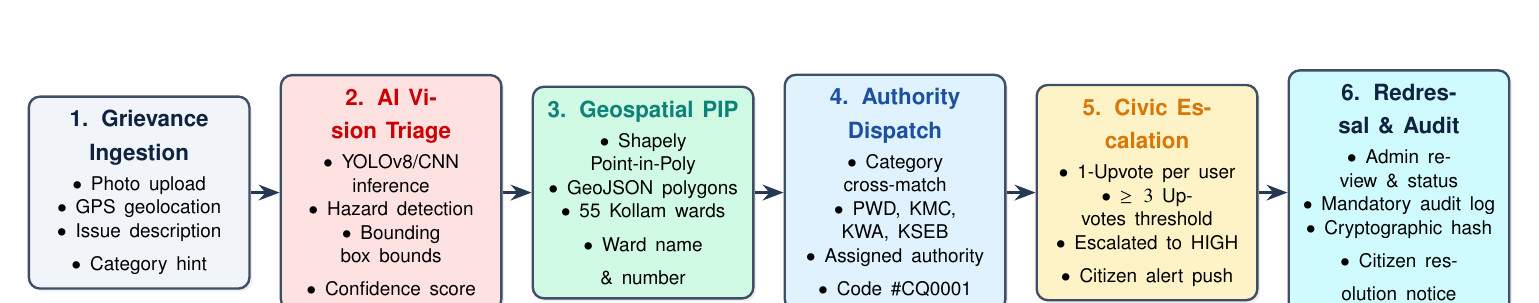
\begin{tikzpicture}[
    x=1cm, y=1cm,
    font=\sffamily,
    stepbox/.style={
        rectangle, draw=civNavy!80, line width=0.85pt, fill=white,
        rounded corners=4pt, inner sep=5pt, align=center,
        drop shadow={shadow xshift=1pt, shadow yshift=-1pt, opacity=0.15}
    },
    flowarr/.style={
        -{Stealth[scale=0.95]}, line width=1.1pt, draw=civNavy!90
    }
]

    % Step 1: Grievance Ingestion
    \node [stepbox, fill=cInput, text width=2.45cm] (p1) at (0, 0) {
        \textbf{\fontsize{8.5}{10.0}\selectfont\color{civNavy}1. Grievance Ingestion}\\[0.25em]
        \fontsize{7.2}{8.5}\selectfont
        $\bullet$ Photo upload\\
        $\bullet$ GPS geolocation\\
        $\bullet$ Issue description\\
        $\bullet$ Category hint
    };

    % Step 2: AI Vision Triage
    \node [stepbox, fill=cStage3, text width=2.45cm] (p2) at (3.20, 0) {
        \textbf{\fontsize{8.5}{10.0}\selectfont\color{red!80!black}2. AI Vision Triage}\\[0.25em]
        \fontsize{7.2}{8.5}\selectfont
        $\bullet$ YOLOv8/CNN inference\\
        $\bullet$ Hazard detection\\
        $\bullet$ Bounding box bounds\\
        $\bullet$ Confidence score
    };

    % Step 3: Geospatial PIP Mapping
    \node [stepbox, fill=cStage1, text width=2.45cm] (p3) at (6.40, 0) {
        \textbf{\fontsize{8.5}{10.0}\selectfont\color{civTeal}3. Geospatial PIP}\\[0.25em]
        \fontsize{7.2}{8.5}\selectfont
        $\bullet$ Shapely Point-in-Poly\\
        $\bullet$ GeoJSON polygons\\
        $\bullet$ 55 Kollam wards\\
        $\bullet$ Ward name \& number
    };

    % Step 4: Authority Dispatch
    \node [stepbox, fill=cStem, text width=2.45cm] (p4) at (9.60, 0) {
        \textbf{\fontsize{8.5}{10.0}\selectfont\color{civBlue}4. Authority Dispatch}\\[0.25em]
        \fontsize{7.2}{8.5}\selectfont
        $\bullet$ Category cross-match\\
        $\bullet$ PWD, KMC, KWA, KSEB\\
        $\bullet$ Assigned authority\\
        $\bullet$ Code \#CQ0001
    };

    % Step 5: Community Escalation
    \node [stepbox, fill=cStage2, text width=2.45cm] (p5) at (12.80, 0) {
        \textbf{\fontsize{8.5}{10.0}\selectfont\color{civGold}5. Civic Escalation}\\[0.25em]
        \fontsize{7.2}{8.5}\selectfont
        $\bullet$ 1-Upvote per user\\
        $\bullet$ $\ge 3$ Upvotes threshold\\
        $\bullet$ Escalated to HIGH\\
        $\bullet$ Citizen alert push
    };

    % Step 6: Resolution & Audit
    \node [stepbox, fill=cStage4, text width=2.45cm] (p6) at (16.00, 0) {
        \textbf{\fontsize{8.5}{10.0}\selectfont\color{civNavy}6. Redressal \& Audit}\\[0.25em]
        \fontsize{7.2}{8.5}\selectfont
        $\bullet$ Admin review \& status\\
        $\bullet$ Mandatory audit log\\
        $\bullet$ Cryptographic hash\\
        $\bullet$ Citizen resolution notice
    };

    % Connecting Flow Arrows
    \draw [flowarr] (p1) -- (p2);
    \draw [flowarr] (p2) -- (p3);
    \draw [flowarr] (p3) -- (p4);
    \draw [flowarr] (p4) -- (p5);
    \draw [flowarr] (p5) -- (p6);

\end{tikzpicture}
\end{document}
}
    \caption{Proposed operational methods pipeline of the CiviQ civic grievance redressal platform.}
    \label{fig:framework}
\end{figure}

\subsection{Layered System Workflow}
Figure~\ref{fig:arch_workflow} illustrates the structured execution lifecycle spanning input acquisition to municipal resolution.

\begin{figure}[H]
    \centering
    \adjustbox{max width=0.98\linewidth, max height=0.72\textheight, keepaspectratio, center}{\documentclass[tikz,border=10pt]{standalone}
\usepackage{tikz}
\usepackage{fontawesome5}
\usetikzlibrary{arrows.meta,positioning,fit,backgrounds,calc,shadows,shapes.geometric}

\definecolor{civNavy}{RGB}{15, 34, 64}
\definecolor{civBlue}{RGB}{28, 80, 160}
\definecolor{civTeal}{RGB}{14, 130, 120}
\definecolor{civLightBlue}{RGB}{238, 245, 255}
\definecolor{civBorder}{RGB}{185, 210, 240}
\definecolor{civGold}{RGB}{217, 119, 6}
\definecolor{civGreen}{RGB}{22, 130, 80}
\definecolor{civDark}{RGB}{20, 28, 42}
\definecolor{cInput}{RGB}{240, 246, 255}
\definecolor{cStem}{RGB}{224, 242, 254}
\definecolor{cStage1}{RGB}{209, 250, 229}
\definecolor{cStage2}{RGB}{254, 243, 199}
\definecolor{cStage3}{RGB}{254, 226, 226}
\definecolor{cStage4}{RGB}{236, 254, 255}

\begin{document}
% Complete Layered System Workflow for CiviQ Civic Grievance Platform
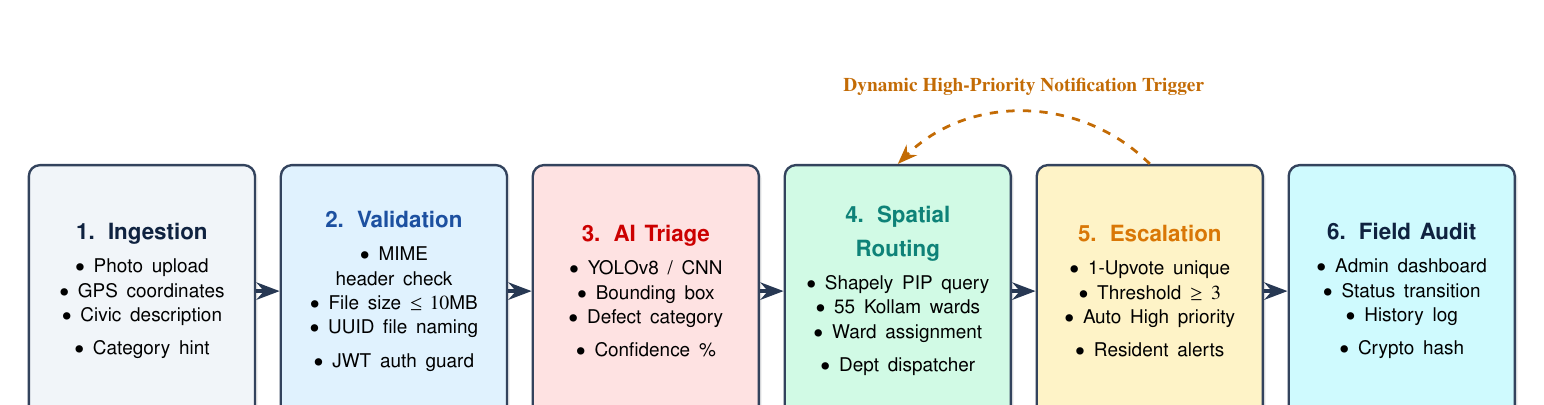
\begin{tikzpicture}[
    x=1cm, y=1cm,
    font=\sffamily,
    stepbox/.style={
        rectangle, draw=civNavy!85, line width=0.85pt, fill=white,
        rounded corners=4pt, inner sep=6pt, align=center,
        minimum height=3.2cm, text width=2.45cm,
        drop shadow={shadow xshift=1pt, shadow yshift=-1pt, opacity=0.15}
    },
    flowarr/.style={
        -{Stealth[scale=1.0]}, line width=1.2pt, draw=civNavy!90
    },
    dashloop/.style={
        -{Stealth[scale=0.95]}, line width=1.0pt, dashed, draw=civGold!90!black
    }
]

    % Step 1: Grievance Ingestion
    \node [stepbox, fill=cInput] (b1) at (0, 0) {
        \textbf{\fontsize{8.5}{10.0}\selectfont\color{civNavy}1. Ingestion}\\[0.35em]
        \fontsize{7.2}{8.8}\selectfont
        $\bullet$ Photo upload\\
        $\bullet$ GPS coordinates\\
        $\bullet$ Civic description\\
        $\bullet$ Category hint
    };

    % Step 2: Validation & Sanitization
    \node [stepbox, fill=cStem] (b2) at (3.2, 0) {
        \textbf{\fontsize{8.5}{10.0}\selectfont\color{civBlue}2. Validation}\\[0.35em]
        \fontsize{7.2}{8.8}\selectfont
        $\bullet$ MIME header check\\
        $\bullet$ File size $\le 10$MB\\
        $\bullet$ UUID file naming\\
        $\bullet$ JWT auth guard
    };

    % Step 3: AI Computer Vision Triage
    \node [stepbox, fill=cStage3] (b3) at (6.4, 0) {
        \textbf{\fontsize{8.5}{10.0}\selectfont\color{red!80!black}3. AI Triage}\\[0.35em]
        \fontsize{7.2}{8.8}\selectfont
        $\bullet$ YOLOv8 / CNN\\
        $\bullet$ Bounding box\\
        $\bullet$ Defect category\\
        $\bullet$ Confidence \%
    };

    % Step 4: Geospatial PIP Routing
    \node [stepbox, fill=cStage1] (b4) at (9.6, 0) {
        \textbf{\fontsize{8.5}{10.0}\selectfont\color{civTeal}4. Spatial Routing}\\[0.35em]
        \fontsize{7.2}{8.8}\selectfont
        $\bullet$ Shapely PIP query\\
        $\bullet$ 55 Kollam wards\\
        $\bullet$ Ward assignment\\
        $\bullet$ Dept dispatcher
    };

    % Step 5: Community Escalation
    \node [stepbox, fill=cStage2] (b5) at (12.8, 0) {
        \textbf{\fontsize{8.5}{10.0}\selectfont\color{civGold}5. Escalation}\\[0.35em]
        \fontsize{7.2}{8.8}\selectfont
        $\bullet$ 1-Upvote unique\\
        $\bullet$ Threshold $\ge 3$\\
        $\bullet$ Auto High priority\\
        $\bullet$ Resident alerts
    };

    % Step 6: Redressal & Audit
    \node [stepbox, fill=cStage4] (b6) at (16.0, 0) {
        \textbf{\fontsize{8.5}{10.0}\selectfont\color{civNavy}6. Field Audit}\\[0.35em]
        \fontsize{7.2}{8.8}\selectfont
        $\bullet$ Admin dashboard\\
        $\bullet$ Status transition\\
        $\bullet$ History log\\
        $\bullet$ Crypto hash
    };

    % Forward Pipeline Arrows
    \draw [flowarr] (b1) -- (b2);
    \draw [flowarr] (b2) -- (b3);
    \draw [flowarr] (b3) -- (b4);
    \draw [flowarr] (b4) -- (b5);
    \draw [flowarr] (b5) -- (b6);

    % Feedback Loop Arrow (Escalation to Redressal)
    \draw [dashloop] (b5.north) to[out=135, in=45] 
        node[above=2pt, font=\fontsize{7.0}{8.5}\selectfont\bfseries, text=civGold!90!black] 
        {Dynamic High-Priority Notification Trigger} (b4.north);

\end{tikzpicture}
\end{document}
}
    \caption{Layered system workflow and 6-stage execution lifecycle across diagnostic and operational layers.}
    \label{fig:arch_workflow}
\end{figure}

\subsection{End-to-End System Flow Architecture}
Figure~\ref{fig:system_flow} delineates the complete end-to-end data transformation pipeline from input acquisition to verified output.

\begin{figure}[H]
    \centering
    \adjustbox{max width=0.98\linewidth, max height=0.72\textheight, keepaspectratio, center}{\documentclass[tikz,border=10pt]{standalone}
\usepackage{tikz}
\usepackage{fontawesome5}
\usepackage{amsmath,amssymb}
\usetikzlibrary{arrows.meta,positioning,fit,backgrounds,calc,shadows,shapes.geometric}

\definecolor{civNavy}{RGB}{15, 34, 64}
\definecolor{civBlue}{RGB}{28, 80, 160}
\definecolor{civTeal}{RGB}{14, 130, 120}
\definecolor{civLightBlue}{RGB}{238, 245, 255}
\definecolor{civBorder}{RGB}{185, 210, 240}
\definecolor{civGold}{RGB}{217, 119, 6}
\definecolor{civGreen}{RGB}{22, 130, 80}
\definecolor{civDark}{RGB}{20, 28, 42}
\definecolor{cInput}{RGB}{240, 246, 255}
\definecolor{cStem}{RGB}{224, 242, 254}
\definecolor{cStage1}{RGB}{209, 250, 229}
\definecolor{cStage2}{RGB}{254, 243, 199}
\definecolor{cStage3}{RGB}{254, 226, 226}
\definecolor{cStage4}{RGB}{236, 254, 255}

\begin{document}
% End-to-End System Flow for CiviQ Platform
\begin{tikzpicture}[
    x=1cm, y=1cm,
    font=\sffamily,
    hdrbox/.style={
        rectangle, draw=civNavy!80, line width=0.85pt, fill=civLightBlue,
        rounded corners=3pt, inner sep=4pt, align=center,
        text width=3.80cm,
        font=\fontsize{8.0}{9.5}\selectfont\bfseries\color{civNavy}
    },
    stepbox/.style={
        rectangle, draw=black!70, line width=0.7pt, fill=white,
        rounded corners=3pt, inner sep=4.0pt, align=center,
        text width=3.80cm,
        font=\fontsize{7.0}{8.2}\selectfont
    },
    enginebox/.style={
        rectangle, draw=civNavy!85, line width=0.85pt, fill=civLightBlue!40,
        rounded corners=3.5pt, inner sep=5.0pt, align=left,
        text width=3.80cm,
        font=\fontsize{6.8}{8.0}\selectfont
    },
    stagebox/.style={
        rectangle, draw=civNavy!40, dashed, rounded corners=5pt, line width=0.8pt,
        fill=civLightBlue!20, inner xsep=5pt, inner ysep=6pt
    },
    flowarr/.style={
        -{Stealth[scale=0.85]}, line width=0.85pt, draw=black!80
    },
    transarr/.style={
        -{Stealth[length=4.5pt, width=3.5pt]}, line width=1.1pt, draw=civBlue
    }
]

    % STAGE 1: INGESTION & GEOTAGGING
    \node[hdrbox] (h1) at (0, 8.4) {\faUser\ Stage 1: Grievance Ingestion};
    \node[stepbox] (s1a) at (0, 7.2) {Citizen Camera / Gallery Upload\\GPS Coordinates \& Category Hint};
    \node[enginebox] (s1b) at (0, 5.1) {\textbf{Frontend UI Components:}\\$\bullet$ Leaflet OpenStreetMap Pin Dropper\\$\bullet$ HTML5 Drag-and-Drop Uploader\\$\bullet$ Description Validation ($\ge 10$ chars)};
    \node[stepbox, fill=cInput] (s1c) at (0, 3.0) {Multipart Form Data Payload\\Image Stream + GPS Coordinates};

    % STAGE 2: API GATEWAY & AI TRIAGE
    \node[hdrbox] (h2) at (4.6, 8.4) {\faRobot\ Stage 2: Gateway \& AI Triage};
    \node[stepbox] (s2a) at (4.6, 7.2) {Flask API Dispatcher \& Auth Token\\MIME Validation \& UUID Persistence};
    \node[enginebox] (s2b) at (4.6, 5.1) {\textbf{Computer Vision Hook:}\\$\bullet$ YOLOv8 / CNN Feature Extraction\\$\bullet$ Hazard Class: Pothole / Waste / Leak\\$\bullet$ Bounding Box Bounds $(t, l, w, h)$\\$\bullet$ AI Confidence Metric ($89\%-97\%$)};
    \node[stepbox, fill=cStage3] (s2c) at (4.6, 3.0) {Categorized Defect Object\\Classified Hazard + Confidence};

    % STAGE 3: GEOSPATIAL PIP & DISPATCH
    \node[hdrbox] (h3) at (9.2, 8.4) {\faRoute\ Stage 3: Spatial Routing};
    \node[stepbox] (s3a) at (9.2, 7.2) {Shapely Point-in-Polygon Engine\\GeoJSON 55 Kollam Ward Boundaries};
    \node[enginebox] (s3b) at (9.2, 5.1) {\textbf{Authority Mapping Engine:}\\$\bullet$ Spatial PIP query: \texttt{.covers()}\\$\bullet$ Ward Name \& Number Resolution\\$\bullet$ Department Cross-Match: PWD / KMC\\$\bullet$ Code Gen: \texttt{\#CQ0001} Sequential Code};
    \node[stepbox, fill=cStage1] (s3c) at (9.2, 3.0) {Municipal Department Assignment\\Responsible Authority Record ID};

    % STAGE 4: REDRESSAL, ESCALATION & AUDIT
    \node[hdrbox] (h4) at (13.8, 8.4) {\faLock\ Stage 4: Redressal \& Audit};
    \node[stepbox] (s4a) at (13.8, 7.2) {MySQL Database Commit \& History\\1-Upvote Constraint \& Community Thread};
    \node[enginebox] (s4b) at (13.8, 5.1) {\textbf{Civic Redressal Lifecycle:}\\$\bullet$ SLA Escalation ($\ge 3$ upvotes $\to$ High)\\$\bullet$ Admin Status Transitions with Remarks\\$\bullet$ Real-time Notification Alert Dispatch\\$\bullet$ Tamper-Evident SHA-256 Crypto Hash};
    \node[stepbox, fill=cStage4] (s4c) at (13.8, 3.0) {Citizen Resolution Receipt\\Audited Lifecycle History Timeline};

    % Background Stage Framing Boxes
    \begin{scope}[on background layer]
        \node[stagebox, fit=(h1) (s1a) (s1b) (s1c)] (box1) {};
        \node[stagebox, fit=(h2) (s2a) (s2b) (s2c)] (box2) {};
        \node[stagebox, fit=(h3) (s3a) (s3b) (s3c)] (box3) {};
        \node[stagebox, fit=(h4) (s4a) (s4b) (s4c)] (box4) {};
    \end{scope}

    % Inter-Stage Transition Arrows
    \draw[transarr] (s1c.east) -- (s2c.west);
    \draw[transarr] (s2c.east) -- (s3c.west);
    \draw[transarr] (s3c.east) -- (s4c.west);

    % Intra-Stage Flow Arrows
    \draw[flowarr] (s1a) -- (s1b);
    \draw[flowarr] (s1b) -- (s1c);
    \draw[flowarr] (s2a) -- (s2b);
    \draw[flowarr] (s2b) -- (s2c);
    \draw[flowarr] (s3a) -- (s3b);
    \draw[flowarr] (s3b) -- (s3c);
    \draw[flowarr] (s4a) -- (s4b);
    \draw[flowarr] (s4b) -- (s4c);

\end{tikzpicture}
\end{document}
}
    \caption{Overall end-to-end system flow architecture from citizen upload to administrative redressal and audit logging.}
    \label{fig:system_flow}
\end{figure}

\section{System Flowchart and Algorithms}

\subsection{System Flowchart}
Figure~\ref{fig:multiagent_flowchart} maps the decision pathways, exception branches, and escalation triggers executing during a grievance request.

\begin{figure}[H]
    \centering
    \adjustbox{max width=0.98\linewidth, max height=0.72\textheight, keepaspectratio, center}{\documentclass[tikz,border=10pt]{standalone}
\usepackage{tikz}
\usepackage{fontawesome5}
\usepackage{amsmath,amssymb}
\usetikzlibrary{arrows.meta,positioning,fit,backgrounds,calc,shadows,shapes.geometric}

\definecolor{civNavy}{RGB}{15, 34, 64}
\definecolor{civBlue}{RGB}{28, 80, 160}
\definecolor{civTeal}{RGB}{14, 130, 120}
\definecolor{civLightBlue}{RGB}{238, 245, 255}
\definecolor{civBorder}{RGB}{185, 210, 240}
\definecolor{civGold}{RGB}{217, 119, 6}
\definecolor{civGreen}{RGB}{22, 130, 80}
\definecolor{civDark}{RGB}{20, 28, 42}
\definecolor{cInput}{RGB}{240, 246, 255}
\definecolor{cStem}{RGB}{224, 242, 254}
\definecolor{cStage1}{RGB}{209, 250, 229}
\definecolor{cStage2}{RGB}{254, 243, 199}
\definecolor{cStage3}{RGB}{254, 226, 226}
\definecolor{cStage4}{RGB}{236, 254, 255}

\begin{document}
% System Operational Flowchart for CiviQ
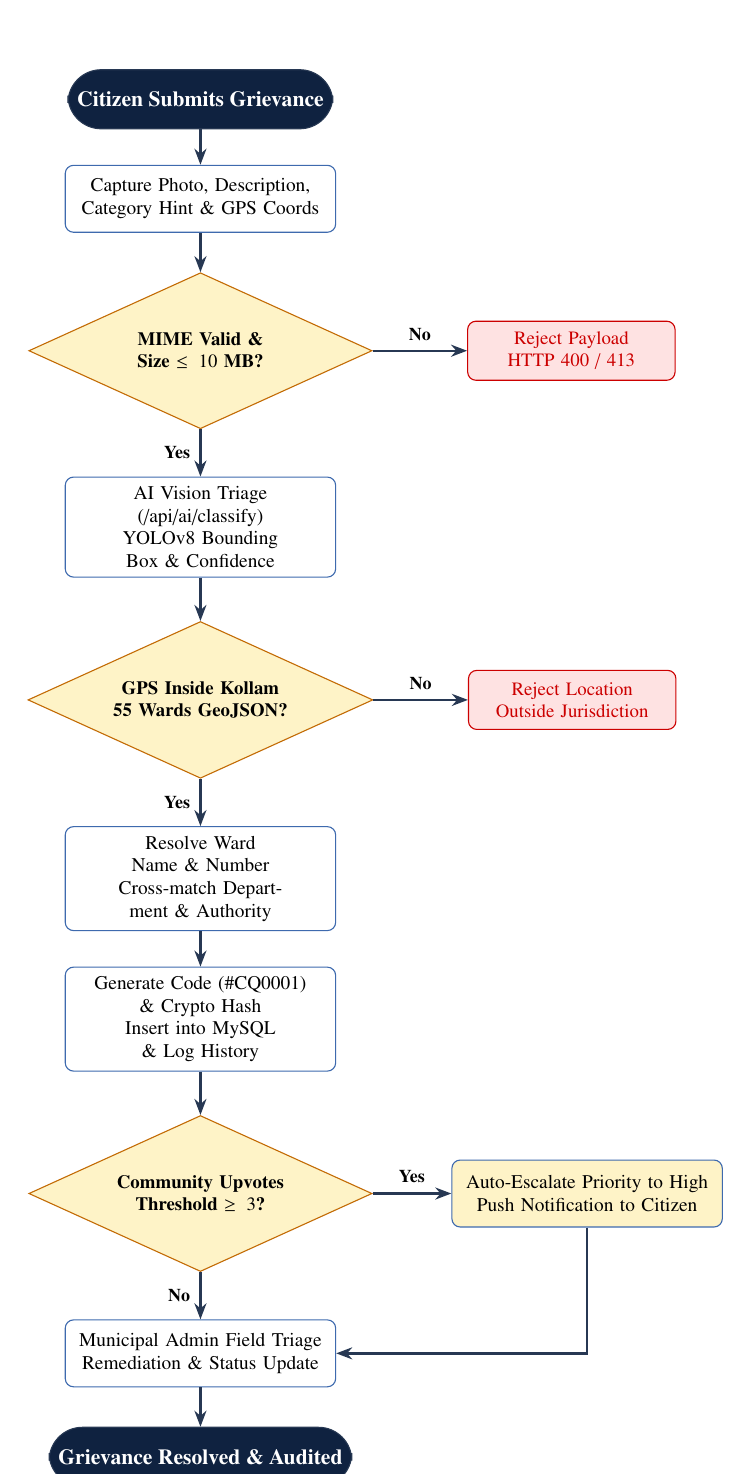
\begin{tikzpicture}[
    x=1cm, y=1cm,
    font=\sffamily,
    startstop/.style={
        rectangle, rounded corners=12pt, minimum width=2.8cm, minimum height=0.75cm,
        text centered, draw=civNavy!90, fill=civNavy, text=white,
        font=\fontsize{7.8}{9.2}\selectfont\bfseries
    },
    process/.style={
        rectangle, rounded corners=3pt, minimum width=3.4cm, minimum height=0.85cm,
        text centered, text width=3.2cm, draw=civBlue!85, fill=white,
        font=\fontsize{7.0}{8.2}\selectfont
    },
    decision/.style={
        diamond, aspect=2.2, minimum width=3.0cm, minimum height=0.9cm,
        text centered, text width=2.6cm, draw=civGold!90!black, fill=cStage2,
        font=\fontsize{6.8}{8.0}\selectfont\bfseries
    },
    errorbox/.style={
        rectangle, rounded corners=3pt, minimum width=2.6cm, minimum height=0.75cm,
        text centered, text width=2.4cm, draw=red!80!black, fill=cStage3,
        font=\fontsize{6.8}{8.0}\selectfont\color{red!80!black}
    },
    flowarr/.style={
        -{Stealth[scale=0.85]}, line width=0.85pt, draw=civNavy!90
    }
]

    % Nodes Placement
    \node (start) [startstop] at (0, 10.2) {Citizen Submits Grievance};
    \node (pingest) [process, below=0.45cm of start] {Capture Photo, Description,\\Category Hint \& GPS Coords};
    
    \node (dmime) [decision, below=0.5cm of pingest] {MIME Valid \&\\Size $\le 10$ MB?};
    \node (errmime) [errorbox, right=1.2cm of dmime] {Reject Payload\\HTTP 400 / 413};

    \node (pai) [process, below=0.6cm of dmime] {AI Vision Triage (/api/ai/classify)\\YOLOv8 Bounding Box \& Confidence};

    \node (dward) [decision, below=0.55cm of pai] {GPS Inside Kollam\\55 Wards GeoJSON?};
    \node (errward) [errorbox, right=1.2cm of dward] {Reject Location\\Outside Jurisdiction};

    \node (proute) [process, below=0.6cm of dward] {Resolve Ward Name \& Number\\Cross-match Department \& Authority};

    \node (pcommit) [process, below=0.45cm of proute] {Generate Code (\#CQ0001) \& Crypto Hash\\Insert into MySQL \& Log History};

    \node (dupvote) [decision, below=0.55cm of pcommit] {Community Upvotes\\Threshold $\ge 3$?};
    \node (pescl) [process, right=1.0cm of dupvote, fill=cStage2] {Auto-Escalate Priority to High\\Push Notification to Citizen};

    \node (padmin) [process, below=0.6cm of dupvote] {Municipal Admin Field Triage\\Remediation \& Status Update};

    \node (stop) [startstop, below=0.5cm of padmin] {Grievance Resolved \& Audited};

    % Arrows
    \draw [flowarr] (start) -- (pingest);
    \draw [flowarr] (pingest) -- (dmime);
    \draw [flowarr] (dmime) -- node[left, font=\fontsize{6.5}{7.5}\selectfont\bfseries] {Yes} (pai);
    \draw [flowarr] (dmime) -- node[above, font=\fontsize{6.5}{7.5}\selectfont\bfseries] {No} (errmime);
    
    \draw [flowarr] (pai) -- (dward);
    \draw [flowarr] (dward) -- node[left, font=\fontsize{6.5}{7.5}\selectfont\bfseries] {Yes} (proute);
    \draw [flowarr] (dward) -- node[above, font=\fontsize{6.5}{7.5}\selectfont\bfseries] {No} (errward);

    \draw [flowarr] (proute) -- (pcommit);
    \draw [flowarr] (pcommit) -- (dupvote);

    \draw [flowarr] (dupvote) -- node[above, font=\fontsize{6.5}{7.5}\selectfont\bfseries] {Yes} (pescl);
    \draw [flowarr] (dupvote) -- node[left, font=\fontsize{6.5}{7.5}\selectfont\bfseries] {No} (padmin);
    \draw [flowarr] (pescl) |- (padmin);

    \draw [flowarr] (padmin) -- (stop);

\end{tikzpicture}
\end{document}
}
    \caption{System flowchart detailing grievance ingestion, MIME validation, AI vision triage, Shapely ward containment, DB insertion, upvote escalation, and administrative redressal.}
    \label{fig:multiagent_flowchart}
\end{figure}

\subsection{System Algorithm}
The complete operational algorithm governing grievance submission, computer vision triage, geospatial routing, community consensus, and administrative resolution is formalized below across twelve sequential steps:

\subsubsection*{Step 1: Grievance Payload Ingestion and MIME Sanitization}
\begin{enumerate}
  \item[\textbf{1.1}] Ingest multipart form payload $\mathcal{F}_{\text{in}}$ containing image stream, location string, GPS coordinates $(\phi, \lambda)$, and description string $\mathcal{D}$.
  \item[\textbf{1.2}] Perform MIME header verification: ensure $\mathrm{MIME}(\mathcal{F}_{\text{in}})$ is in $\{\texttt{image/jpeg},$ $\texttt{image/png},$ $\texttt{image/webp}\}$. If invalid, return HTTP 400.
  \item[\textbf{1.3}] Enforce payload boundary limit: Verify $\mathrm{size}(\mathcal{F}_{\text{in}}) \le 10\,\mathrm{MB}$; return HTTP 413 on violation.
  \item[\textbf{1.4}] Generate unique sanitized filename $f_{\text{name}} = \texttt{"issue\_"} \,\|\, \text{hex}_{12} \,\|\, \texttt{"\_"} \,\|\, \text{name}_{\text{clean}}$ using UUID4 and Werkzeug \texttt{secure\_filename}. Store file under \texttt{backend/uploads/}.
\end{enumerate}

\subsubsection*{Step 2: AI Computer Vision Defect Triage}
\begin{enumerate}
  \item[\textbf{2.1}] Forward sanitized image to AI triage endpoint (\texttt{POST /api/ai/classify}).
  \item[\textbf{2.2}] Execute convolutional feature extraction and evaluate classification score across defect taxonomies $\mathcal{C}$.
  \item[\textbf{2.3}] Compute normalized spatial bounding box coordinates $\hat{\mathcal{B}} = [x_{\text{top}}, y_{\text{left}}, w, h]$ and confidence percentage $\kappa \in [89\%, 97\%]$.
  \item[\textbf{2.4}] Extract suggested department routing hint corresponding to detected category (e.g., Pothole $\to$ PWD, Garbage $\to$ Sanitation).
\end{enumerate}

\subsubsection*{Step 3: Geospatial Coordinate Ingestion and Point Validation}
\begin{enumerate}
  \item[\textbf{3.1}] Validate latitude $\phi$ and longitude $\lambda$: Ensure $-90 \le \phi \le 90$ and $-180 \le \lambda \le 180$.
  \item[\textbf{3.2}] Formulate Shapely two-dimensional geometric point object: $\mathbf{p} = \mathrm{Point}(\lambda, \phi)$.
\end{enumerate}

\subsubsection*{Step 4: Shapely Point-in-Polygon Ward Resolution}
\begin{enumerate}
  \item[\textbf{4.1}] Open and parse GeoJSON boundary dataset \texttt{backend/data/} \allowbreak \texttt{kollam\_ward.json}.
  \item[\textbf{4.2}] Iterate over all 55 ward features. Extract polygon geometry and evaluate $\mathrm{ward\_polygon.covers}(\mathbf{p})$.
  \item[\textbf{4.3}] If a covering polygon is detected, extract feature properties: Ward Number $N_w$, Ward Name $S_w$, District, and Local Body. Format string: $W_{\text{desc}} = \texttt{"Ward "} \,\|\, N_w \,\|\, \texttt{" ("} \,\|\, S_w \,\|\, \texttt{")"}$.
  \item[\textbf{4.4}] If no covering polygon matches, reject submission with HTTP 400: \textit{``Location outside available Kollam Corporation ward map.''}
\end{enumerate}

\subsubsection*{Step 5: Automated Department and Authority Cross-Matching}
\begin{enumerate}
  \item[\textbf{5.1}] Query MySQL \texttt{authorities} table matching detected category department scope (Roads $\to$ PWD, Waste $\to$ Health/Sanitation, Water $\to$ KWA, Lighting $\to$ KSEB) and resolved ward $W_{\text{desc}}$.
  \item[\textbf{5.2}] Retrieve assigned authority primary key $A_{\text{id}}$ and official department name $D_{\text{name}}$.
  \item[\textbf{5.3}] If no ward-specific cell exists, fallback to central municipal zonal engineering office.
\end{enumerate}

\subsubsection*{Step 6: Sequential Grievance Tracking Code Generation}
\begin{enumerate}
  \item[\textbf{6.1}] Execute atomic query counting existing records: $N_{\text{total}} = \mathrm{Count}(\texttt{complaints})$.
  \item[\textbf{6.2}] Generate formatted sequential identifier: $\mathrm{Code} = \texttt{"\#CQ"} \,\|\, \mathrm{PadZeroes}(N_{\text{total}} + 1, 4)$.
\end{enumerate}

\subsubsection*{Step 7: Cryptographic Hash Generation and Database Insertion}
\begin{enumerate}
  \item[\textbf{7.1}] Compute simulated Ethereum-style hexadecimal transaction hash $H_{\text{tx}} = \texttt{"0x"} \,\|\, \mathrm{HexRand}(40)$ and block height $B_n = 18455200 + \mathrm{Rand}(10, 999)$.
  \item[\textbf{7.2}] Execute SQL insert into \texttt{complaints} storing title, category, description, coordinates, ward, authority ID, status \texttt{"Pending"}, priority \texttt{"Medium"}, and initial upvote count 1.
  \item[\textbf{7.3}] Insert initial upvote into \texttt{upvotes} table binding reporting citizen $u_{\text{id}}$ to complaint ID.
\end{enumerate}

\subsubsection*{Step 8: Audit History Logging and Citizen Notification Dispatch}
\begin{enumerate}
  \item[\textbf{8.1}] Insert initial lifecycle entry into \texttt{complaint\_history} with $\mathrm{OldStatus} = \texttt{"Submitted"}$, $\mathrm{NewStatus} = \texttt{"Pending"}$, and $\mathrm{Remarks}$ recording dispatch to department $D_{\text{name}}$.
  \item[\textbf{8.2}] Insert notification record into \texttt{notifications} alerting citizen of successful registration.
\end{enumerate}

\subsubsection*{Step 9: Community Upvoting and Anti-Duplication Enforcement}
\begin{enumerate}
  \item[\textbf{9.1}] When a community resident submits an upvote request (\texttt{POST /api/complaints/<id>/upvote}), verify citizen authentication.
  \item[\textbf{9.2}] Query \texttt{upvotes} table for existing $(u_{\text{id}}, c_{\text{id}})$. If found, reject with HTTP 400: \textit{``You have already upvoted this complaint.''}
  \item[\textbf{9.3}] Atomically insert $(u_{\text{id}}, c_{\text{id}})$ into \texttt{upvotes} and increment complaint counter: $u_{\text{new}} = u_{\text{old}} + 1$.
\end{enumerate}

\subsubsection*{Step 10: Dynamic SLA and Priority Escalation Execution}
\begin{enumerate}
  \item[\textbf{10.1}] Check if updated upvote tally $u_{\text{new}} \ge \tau_{\text{up}}$ (threshold 3) and current priority $\in \{\text{Low}, \text{Medium}\}$.
  \item[\textbf{10.2}] If threshold is satisfied, escalate priority to \texttt{"High"}.
  \item[\textbf{10.3}] Dispatch immediate escalation notification to complaint owner and log escalation in history.
\end{enumerate}

\subsubsection*{Step 11: Administrative Triage and Status Transition}
\begin{enumerate}
  \item[\textbf{11.1}] Municipal official inspects complaints via administrative portal (\texttt{GET /api/admin/complaints}).
  \item[\textbf{11.2}] When official submits a status update via \texttt{PATCH /api/admin/} \allowbreak \texttt{complaints/<id>/status}, validate official role (\texttt{@admin\_required}).
  \item[\textbf{11.3}] Update complaint status to \texttt{"Under Review"}, \texttt{"In Progress"}, \texttt{"Resolved"}, or \texttt{"Rejected"}.
  \item[\textbf{11.4}] Insert mandatory audit entry into \texttt{complaint\_history} with official's user ID and remarks.
\end{enumerate}

\subsubsection*{Step 12: Telemetry Synchronization and CSV Export}
\begin{enumerate}
  \item[\textbf{12.1}] Recalculate municipal department SLA metrics: $\mathrm{Rate}_{\text{res}} = (\mathrm{Resolved} / \mathrm{Total}) \times 100\%$.
  \item[\textbf{12.2}] Update Leaflet OpenStreetMap markers and cluster popups across active citizen clients.
  \item[\textbf{12.3}] Stream complete complaint registers upon demand via streaming CSV endpoint (\texttt{GET /api/admin/export-csv}).
\end{enumerate}

\subsection{Complaint Lifecycle State Transition Graph}
Figure~\ref{fig:dag_scheduling_walkthrough} illustrates the state transition lifecycle and escalation graph governing complaint statuses.

\begin{figure}[H]
    \centering
    \adjustbox{max width=0.98\linewidth, max height=0.68\textheight, keepaspectratio, center}{\documentclass[tikz,border=10pt]{standalone}
\usepackage{tikz}
\usepackage{fontawesome5}
\usepackage{amsmath,amssymb}
\usetikzlibrary{arrows.meta,positioning,fit,backgrounds,calc,shadows,shapes.geometric}

\definecolor{civNavy}{RGB}{15, 34, 64}
\definecolor{civBlue}{RGB}{28, 80, 160}
\definecolor{civTeal}{RGB}{14, 130, 120}
\definecolor{civLightBlue}{RGB}{238, 245, 255}
\definecolor{civGold}{RGB}{217, 119, 6}
\definecolor{civGreen}{RGB}{22, 130, 80}
\definecolor{civRed}{RGB}{220, 38, 38}
\definecolor{cInput}{RGB}{240, 246, 255}
\definecolor{cStem}{RGB}{224, 242, 254}
\definecolor{cStage1}{RGB}{209, 250, 229}
\definecolor{cStage2}{RGB}{254, 243, 199}
\definecolor{cStage3}{RGB}{254, 226, 226}
\definecolor{cStage4}{RGB}{236, 254, 255}

\begin{document}
% Complaint Lifecycle State Machine & Escalation DAG for CiviQ
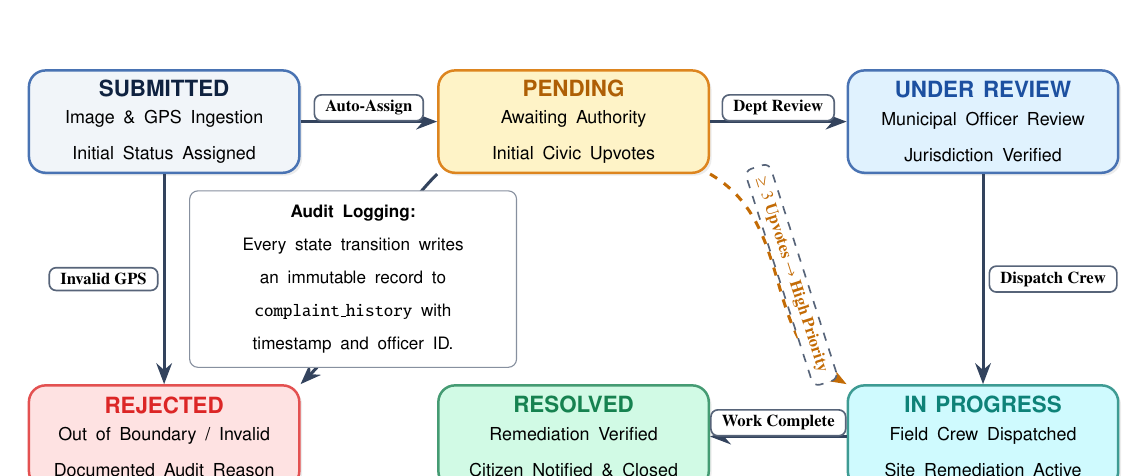
\begin{tikzpicture}[
    x=1cm, y=1cm,
    font=\sffamily,
    every node/.style={align=center},
    statebox/.style={
        rectangle, rounded corners=6pt, minimum width=3.4cm, minimum height=1.3cm,
        text width=3.2cm, align=center, line width=0.9pt, draw=civNavy!80, fill=white,
        drop shadow={shadow xshift=1pt, shadow yshift=-1pt, opacity=0.15}
    },
    transarr/.style={
        -{Stealth[scale=0.95]}, line width=1.1pt, draw=civNavy!85
    },
    esclarr/.style={
        -{Stealth[scale=0.95]}, line width=1.1pt, dashed, draw=civGold!90!black
    },
    auditbadge/.style={
        rectangle, rounded corners=2.5pt, fill=white, draw=civNavy!70, line width=0.6pt,
        inner xsep=4pt, inner ysep=2pt, font=\fontsize{6.0}{7.0}\selectfont\bfseries,
        align=center
    }
]

    % State Nodes
    \node (ssub) [statebox, fill=cInput, draw=civBlue!80] at (0, 6.0) {%
        \textbf{\fontsize{8.5}{10.0}\selectfont\color{civNavy}SUBMITTED}\\[0.2em]
        {\fontsize{6.8}{8.0}\selectfont Image \& GPS Ingestion\\[1pt]Initial Status Assigned}%
    };

    \node (spen) [statebox, fill=cStage2, draw=civGold!90] at (5.2, 6.0) {%
        \textbf{\fontsize{8.5}{10.0}\selectfont\color{civGold!80!black}PENDING}\\[0.2em]
        {\fontsize{6.8}{8.0}\selectfont Awaiting Authority\\[1pt]Initial Civic Upvotes}%
    };

    \node (srev) [statebox, fill=cStem, draw=civBlue!80] at (10.4, 6.0) {%
        \textbf{\fontsize{8.5}{10.0}\selectfont\color{civBlue}UNDER REVIEW}\\[0.2em]
        {\fontsize{6.8}{8.0}\selectfont Municipal Officer Review\\[1pt]Jurisdiction Verified}%
    };

    \node (sprog) [statebox, fill=cStage4, draw=civTeal!80] at (10.4, 2.0) {%
        \textbf{\fontsize{8.5}{10.0}\selectfont\color{civTeal}IN PROGRESS}\\[0.2em]
        {\fontsize{6.8}{8.0}\selectfont Field Crew Dispatched\\[1pt]Site Remediation Active}%
    };

    \node (sres) [statebox, fill=cStage1, draw=civGreen!80] at (5.2, 2.0) {%
        \textbf{\fontsize{8.5}{10.0}\selectfont\color{civGreen}RESOLVED}\\[0.2em]
        {\fontsize{6.8}{8.0}\selectfont Remediation Verified\\[1pt]Citizen Notified \& Closed}%
    };

    \node (srej) [statebox, fill=cStage3, draw=civRed!80] at (0, 2.0) {%
        \textbf{\fontsize{8.5}{10.0}\selectfont\color{civRed}REJECTED}\\[0.2em]
        {\fontsize{6.8}{8.0}\selectfont Out of Boundary / Invalid\\[1pt]Documented Audit Reason}%
    };

    % Transitions
    \draw [transarr] (ssub) -- node[above, auditbadge] {Auto-Assign} (spen);
    \draw [transarr] (spen) -- node[above, auditbadge] {Dept Review} (srev);
    \draw [transarr] (srev) -- node[right=2pt, auditbadge] {Dispatch Crew} (sprog);
    \draw [transarr] (sprog) -- node[above, auditbadge] {Work Complete} (sres);
    \draw [transarr] (ssub) -- node[left=2pt, auditbadge] {Invalid GPS} (srej);
    \draw [transarr] (spen.south west) to[out=225, in=45] node[pos=0.5, above, auditbadge, sloped] {Reject Claim} (srej.north east);

    % Escalation Path (from Pending to In Progress)
    \draw [esclarr] (spen.south east) to[out=-30, in=150] 
        node[pos=0.5, above, auditbadge, sloped, text=civGold!90!black] 
        {$\ge 3$ Upvotes $\rightarrow$ High Priority} (sprog.north west);

    % Legend Box in left-center zone (completely away from escalation arrow)
    \node (legend) [rectangle, draw=civNavy!50, rounded corners=3pt, fill=white, inner sep=5pt, align=center, text width=3.8cm] at (2.4, 4.0) {%
      {\fontsize{6.5}{7.8}\selectfont\textbf{Audit Logging:}\\Every state transition writes an immutable record to \texttt{complaint\_history} with timestamp and officer ID.}%
    };

\end{tikzpicture}
\end{document}
}
    \caption{Complaint lifecycle state transition and escalation DAG illustrating states, transitions, escalation pathways, and audit logging.}
    \label{fig:dag_scheduling_walkthrough}
\end{figure}

\section{Database Design and Schema Connectors}

\subsection{Relational Entity Schema Connectors}
Figure~\ref{fig:db_schema} depicts the 7-table relational schema architecture connecting users, complaints, authorities, upvotes, comments, notifications, and complaint history.

\begin{figure}[H]
    \centering
    \adjustbox{max width=0.98\linewidth, max height=0.72\textheight, keepaspectratio, center}{\documentclass[tikz,border=12pt]{standalone}
\usepackage{tikz}
\usepackage{fontawesome5}
\usetikzlibrary{shapes.multipart,shadows,arrows.meta,positioning,calc}

\definecolor{civNavy}{RGB}{18, 38, 70}
\definecolor{civBlue}{RGB}{24, 76, 155}
\definecolor{civLightBlue}{RGB}{240, 246, 255}
\definecolor{civLine}{RGB}{28, 80, 160}

\begin{document}
% Relational Entity Schema Connectors for CiviQ Database
\begin{tikzpicture}[
    x=1cm, y=1cm,
    font=\sffamily,
    entity/.style={
        rectangle split,
        rectangle split parts=2,
        rectangle split part fill={civNavy, white},
        draw=civNavy,
        line width=0.85pt,
        rounded corners=3.5pt,
        drop shadow={shadow xshift=1.2pt, shadow yshift=-1.2pt, opacity=0.12},
        inner sep=4.5pt,
        align=left
    },
    hubEntity/.style={
        rectangle split,
        rectangle split parts=2,
        rectangle split part fill={civBlue, white},
        draw=civBlue,
        line width=0.95pt,
        rounded corners=3.5pt,
        drop shadow={shadow xshift=1.5pt, shadow yshift=-1.5pt, opacity=0.15},
        inner sep=4.8pt,
        align=left
    },
    fkarr/.style={
        -{Stealth[scale=0.85]}, line width=0.9pt, draw=civLine
    },
    cardlabel/.style={
        font=\fontsize{6.2}{7.4}\selectfont\bfseries,
        fill=white,
        draw=civLine!50,
        text=civNavy,
        line width=0.5pt,
        inner sep=1.8pt,
        rounded corners=2pt
    }
]

    %==========================================================================
    % TIER 1: PARENT ENTITIES (users & authorities)
    %==========================================================================
    
    % TABLE 1: USERS (Top Left)
    \node [entity, text width=3.7cm, anchor=north] (users) at (2.2, 11.5) {
        \centering\textcolor{white}{\textbf{\fontsize{7.5}{9.0}\selectfont\faUsers\ users}}
        \nodepart{two}
        \fontsize{6.2}{7.6}\selectfont
        \underline{\textbf{id}} : INT (PK, Auto)\\[2pt]
        \textbf{name} : VARCHAR(150)\\[2pt]
        \textbf{email} : VARCHAR(150) (UQ)\\[2pt]
        \textbf{password\_hash} : VARCHAR(255)\\[2pt]
        \textbf{role} : ENUM('Citizen', 'Admin')\\[2pt]
        \textbf{ward} : VARCHAR(100)\\[2pt]
        \textbf{created\_at} : TIMESTAMP
    };

    % TABLE 2: AUTHORITIES (Top Right)
    \node [entity, text width=3.7cm, anchor=north] (auth) at (11.8, 11.5) {
        \centering\textcolor{white}{\textbf{\fontsize{7.5}{9.0}\selectfont\faBuilding\ authorities}}
        \nodepart{two}
        \fontsize{6.2}{7.6}\selectfont
        \underline{\textbf{id}} : INT (PK, Auto)\\[2pt]
        \textbf{name} : VARCHAR(150)\\[2pt]
        \textbf{department} : VARCHAR(100)\\[2pt]
        \textbf{jurisdiction} : ENUM(...)\\[2pt]
        \textbf{ward} : VARCHAR(100)\\[2pt]
        \textbf{district} : VARCHAR(100)\\[2pt]
        \textbf{is\_active} : BOOLEAN
    };

    %==========================================================================
    % TIER 2: CENTRAL CORE HUB (complaints)
    %==========================================================================
    
    \node [hubEntity, text width=5.2cm, anchor=north] (comp) at (7.0, 7.4) {
        \centering\textcolor{white}{\textbf{\fontsize{8.0}{9.5}\selectfont\faFile\ complaints}}
        \nodepart{two}
        \fontsize{6.2}{7.6}\selectfont
        \underline{\textbf{id}} : INT (PK, Auto)\\[1.8pt]
        \textbf{complaint\_id\_code} : VARCHAR(30) (UQ)\\[1.8pt]
        \textbf{user\_id} : INT (FK $\to$ users.id)\\[1.8pt]
        \textbf{title} : VARCHAR(200)\\[1.8pt]
        \textbf{description} : TEXT\\[1.8pt]
        \textbf{category} : VARCHAR(100)\\[1.8pt]
        \textbf{location\_address} : VARCHAR(255)\\[1.8pt]
        \textbf{latitude, longitude} : DECIMAL(10, 7)\\[1.8pt]
        \textbf{ward} : VARCHAR(100)\\[1.8pt]
        \textbf{authority\_id} : INT (FK $\to$ authorities.id)\\[1.8pt]
        \textbf{status} : ENUM('Pending', 'In Progress', ...)\\[1.8pt]
        \textbf{priority} : ENUM('Low', 'Medium', 'High')\\[1.8pt]
        \textbf{upvote\_count} : INT DEFAULT 0\\[1.8pt]
        \textbf{ai\_confidence} : VARCHAR(20)
    };

    %==========================================================================
    % TIER 3: CHILD AUXILIARY TABLES (4 across the bottom)
    %==========================================================================
    
    % TABLE 4: UPVOTES (Leftmost)
    \node [entity, text width=2.85cm, anchor=north] (upvotes) at (1.8, 0.2) {
        \centering\textcolor{white}{\textbf{\fontsize{7.2}{8.5}\selectfont\faThumbsUp\ upvotes}}
        \nodepart{two}
        \fontsize{6.2}{7.6}\selectfont
        \underline{\textbf{id}} : INT (PK)\\[2pt]
        \textbf{user\_id} : INT (FK)\\[2pt]
        \textbf{complaint\_id} : INT (FK)\\[2pt]
        \textbf{created\_at} : TIMESTAMP\\[2pt]
        \textit{UQ (user\_id, complaint\_id)}
    };

    % TABLE 5: COMMENTS (Center-Left)
    \node [entity, text width=2.85cm, anchor=north] (comments) at (5.25, 0.2) {
        \centering\textcolor{white}{\textbf{\fontsize{7.2}{8.5}\selectfont\faComments\ comments}}
        \nodepart{two}
        \fontsize{6.2}{7.6}\selectfont
        \underline{\textbf{id}} : INT (PK)\\[2pt]
        \textbf{complaint\_id} : INT (FK)\\[2pt]
        \textbf{user\_id} : INT (FK)\\[2pt]
        \textbf{comment\_text} : TEXT\\[2pt]
        \textbf{created\_at} : TIMESTAMP
    };

    % TABLE 6: NOTIFICATIONS (Center-Right)
    \node [entity, text width=2.85cm, anchor=north] (notif) at (8.75, 0.2) {
        \centering\textcolor{white}{\textbf{\fontsize{7.2}{8.5}\selectfont\faBell\ notifications}}
        \nodepart{two}
        \fontsize{6.2}{7.6}\selectfont
        \underline{\textbf{id}} : INT (PK)\\[2pt]
        \textbf{user\_id} : INT (FK)\\[2pt]
        \textbf{complaint\_id} : INT (FK)\\[2pt]
        \textbf{title} : VARCHAR(150)\\[2pt]
        \textbf{is\_read} : BOOLEAN
    };

    % TABLE 7: COMPLAINT HISTORY (Rightmost)
    \node [entity, text width=2.85cm, anchor=north] (hist) at (12.2, 0.2) {
        \centering\textcolor{white}{\textbf{\fontsize{7.2}{8.5}\selectfont\faHistory\ complaint\_history}}
        \nodepart{two}
        \fontsize{6.2}{7.6}\selectfont
        \underline{\textbf{id}} : INT (PK)\\[2pt]
        \textbf{complaint\_id} : INT (FK)\\[2pt]
        \textbf{changed\_by\_user} : INT\\[2pt]
        \textbf{old\_status, new\_status}\\[2pt]
        \textbf{created\_at} : TIMESTAMP
    };

    %==========================================================================
    % CONNECTIONS & RELATIONSHIPS
    %==========================================================================
    
    % Tier 1 to Tier 2: Clean Orthogonal Routes into exact FK attributes
    % user_id in complaints is at y ~ 6.5
    \draw [fkarr] (users.south) -- (2.2, 6.5) -- node[midway, above, cardlabel] {1 : N} ([yshift=-25pt]comp.north west);

    % authority_id in complaints is at y ~ 3.8
    \draw [fkarr] (auth.south) -- (11.8, 3.8) -- node[midway, above, cardlabel] {1 : N} ([yshift=-100pt]comp.north east);

    % Tier 2 to Tier 3: Orthogonal Distribution Bus in Clear Air at y=0.9
    \draw [line width=0.9pt, draw=civLine] (comp.south) -- (7.0, 0.9);
    \draw [line width=0.9pt, draw=civLine] (1.8, 0.9) -- (12.2, 0.9);

    % Drop Arrows from Bus into Child Tables
    \draw [fkarr] (1.8, 0.9) -- (upvotes.north);
    \draw [fkarr] (5.25, 0.9) -- (comments.north);
    \draw [fkarr] (8.75, 0.9) -- (notif.north);
    \draw [fkarr] (12.2, 0.9) -- (hist.north);

    % Cardinality Badges on Bus
    \node [cardlabel] at (7.0, 1.25) {1};
    \node [cardlabel] at (1.8, 0.55) {N};
    \node [cardlabel] at (5.25, 0.55) {N};
    \node [cardlabel] at (8.75, 0.55) {N};
    \node [cardlabel] at (12.2, 0.55) {N};

\end{tikzpicture}
\end{document}
}
    \caption{Relational entity and database schema connectors showing 7 normalized tables, primary/foreign keys, and relational cardinality.}
    \label{fig:db_schema}
\end{figure}

\clearpage
\enlargethispage{2\baselineskip}
\subsection{Level-1 Data Flow Architecture}
Figure~\ref{fig:data_flow_diagram} illustrates the Level-1 Data Flow Diagram (DFD), showing external entities, primary processing transformations, datastores, and feedback loops.

\begin{figure}[H]
    \centering
    \vspace{-4pt}
    \adjustbox{max width=0.98\linewidth, max height=0.42\textheight, keepaspectratio, center}{\documentclass[tikz,border=10pt]{standalone}
\usepackage{tikz}
\usepackage{fontawesome5}
\usetikzlibrary{arrows.meta,positioning,fit,backgrounds,calc,shadows,shapes.geometric}

\definecolor{civNavy}{RGB}{15, 34, 64}
\definecolor{civBlue}{RGB}{28, 80, 160}
\definecolor{civTeal}{RGB}{14, 130, 120}
\definecolor{civLightBlue}{RGB}{238, 245, 255}
\definecolor{civBorder}{RGB}{185, 210, 240}
\definecolor{civGold}{RGB}{217, 119, 6}
\definecolor{civGreen}{RGB}{22, 130, 80}
\definecolor{civDark}{RGB}{20, 28, 42}
\definecolor{cInput}{RGB}{240, 246, 255}
\definecolor{cStem}{RGB}{224, 242, 254}
\definecolor{cStage1}{RGB}{209, 250, 229}

\begin{document}
% Level-1 Data Flow Diagram (DFD) for CiviQ Platform
\begin{tikzpicture}[
    x=1cm, y=1cm,
    font=\sffamily,
    entity/.style={
        rectangle, draw=civNavy, line width=1.1pt, fill=white,
        rounded corners=3.5pt, minimum width=2.6cm, minimum height=1.15cm,
        align=center, font=\fontsize{8.5}{10.0}\selectfont\bfseries,
        drop shadow={shadow xshift=1.2pt, shadow yshift=-1.2pt, opacity=0.15}
    },
    process/.style={
        circle, draw=civNavy, line width=1.1pt, fill=cInput,
        minimum size=1.85cm, align=center,
        font=\fontsize{7.5}{8.8}\selectfont\bfseries,
        drop shadow={shadow xshift=1pt, shadow yshift=-1pt, opacity=0.12}
    },
    datastore/.style={
        rectangle, draw=civNavy!90, line width=0.95pt, fill=cStage1,
        minimum width=2.8cm, minimum height=0.85cm, align=center,
        font=\fontsize{7.5}{8.8}\selectfont\bfseries,
        drop shadow={shadow xshift=1pt, shadow yshift=-1pt, opacity=0.10}
    },
    dfdarr/.style={
        -{Stealth[scale=0.95]}, line width=0.95pt, draw=civNavy!90
    },
    flowlabel/.style={
        font=\fontsize{6.5}{7.5}\selectfont\bfseries, fill=white,
        draw=civNavy!25, line width=0.4pt, inner sep=2.0pt, rounded corners=2pt
    }
]

    % Row 1: Entities & Top Processes (y=7.2)
    \node (ecitizen) [entity] at (1.2, 7.2) {\faUser\ Citizen};
    \node (p1) [process] at (4.5, 7.2) {1.0\\Auth \&\\Profiles};
    \node (p5) [process] at (8.2, 7.2) {5.0\\Redressal\\\& Audit};
    \node (eadmin) [entity] at (11.8, 7.2) {\faUserShield\ Municipal\\Admin};

    % Row 2: Users Datastore (y=5.5)
    \node (d1) [datastore] at (4.5, 5.5) {D1: Users DB};

    % Row 3: Processing Core & Central Complaints Store (y=3.8)
    \node (p2) [process] at (1.2, 3.8) {2.0\\AI Vision\\Triage};
    \node (p3) [process] at (4.5, 3.8) {3.0\\GIS Ward\\Routing};
    \node (d2) [datastore, minimum width=2.9cm] at (8.2, 3.8) {D2: Complaints DB};
    \node (d6) [datastore] at (11.8, 3.8) {D6: Audit History Log};

    % Row 4: Spatial & Authority Datastores (y=2.2)
    \node (d3) [datastore] at (4.5, 2.2) {D3: GeoJSON Wards};
    \node (d4) [datastore] at (8.2, 2.2) {D4: Authorities DB};

    % Row 5: Civic Upvoting Process & Ledger (y=0.6)
    \node (p4) [process] at (1.2, 0.6) {4.0\\Civic\\Consensus};
    \node (d5) [datastore] at (4.5, 0.6) {D5: Upvotes DB};

    % Connections - Authentication Tier
    \draw [dfdarr] (ecitizen) -- node[above, flowlabel] {Credentials} (p1);
    \draw [dfdarr] (p1) -- node[right, flowlabel] {User Record} (d1);

    % Connections - Grievance Ingestion & AI Triage Tier
    \draw [dfdarr] (ecitizen) -- node[right, flowlabel] {Photo + GPS} (p2);
    \draw [dfdarr] (p2) -- node[above, flowlabel] {Defect Class} (p3);

    % Connections - Spatial Containment & Department Dispatch
    \draw [dfdarr] (d3) -- node[right, flowlabel] {Ward Polygons} (p3);
    \draw [dfdarr] (d4) -- node[right, flowlabel] {Dept Scopes} (d2);
    \draw [dfdarr] (p3) -- node[above, flowlabel] {Routed Issue} (d2);

    % Connections - Community Consensus Tier
    \draw [dfdarr] (p2) -- node[right, flowlabel] {Upvote Claim} (p4);
    \draw [dfdarr] (p4) -- node[above, flowlabel] {1-Upvote Unique} (d5);
    \draw [dfdarr] (p4.south) -- ++(0, -0.45) -| node[pos=0.3, above, flowlabel] {Priority Escalation ($\ge 3$)} (d2.south);

    % Connections - Municipal Redressal & Audit Trail Tier
    \draw [dfdarr] (d2) -- node[right, flowlabel] {Complaint State} (p5);
    \draw [dfdarr] (eadmin) -- node[above, flowlabel] {Status Update} (p5);
    \draw [dfdarr] (p5.south) to[out=-40, in=140] node[pos=0.45, above=2pt, flowlabel] {Audit Event Log} (d6.north west);

\end{tikzpicture}
\end{document}
}
    \vspace{-4pt}
    \caption{Level-1 Data Flow Diagram (DFD) depicting external entities, processing stages, datastores, and notification feedback loops.}
    \label{fig:data_flow_diagram}
\end{figure}

\vspace{-4pt}
\subsubsection{Process Transformation and Data Flow Analysis}
The platform dataflow formalizes five primary computational transformations and feedback loops:

\begin{enumerate}[1.]\setlength{\itemsep}{0.5pt}\setlength{\parsep}{0pt}\setlength{\topsep}{1pt}
    \item \textbf{Process 1.0 (Auth \& Profiles):} Validates credentials via PBKDF2-HMAC-SHA256, issues signed JWT tokens, and maps session claims to \texttt{D1: Users DB}.
    \item \textbf{Process 2.0 (AI Vision Triage):} Sanitizes images ($\le 5$\,MB) and executes YOLOv8 inference to classify civic defects with prediction confidence scores.
    \item \textbf{Process 3.0 (GIS Ward Routing):} Executes Point-in-Polygon ray-casting across 55 Kollam wards in \texttt{D3}, resolving authorities via \texttt{D4} to persist complaints in \texttt{D2}.
    \item \textbf{Process 4.0 (Civic Consensus):} Validates unique upvotes in \texttt{D5: Upvotes DB}, triggering priority escalation to \textit{High} in \texttt{D2} once $\ge 3$ endorsements are reached.
    \item \textbf{Process 5.0 (Redressal \& Audit):} Coordinates status updates (\textit{Pending} $\to$ \textit{In Progress} $\to$ \textit{Resolved}), logging immutable audit rows in \texttt{D6} and dispatching citizen notifications.
\end{enumerate}


%==============================================================================
% CHAPTER 6: DESIGN AND METHODOLOGY
%==============================================================================
\chapter{Design and Methodology}

This chapter expounds the mathematical formulations, algorithmic implementations, geospatial analysis, authority routing, and experimental integration testing governing the CiviQ platform.

\section{AI Vision Triage and Geospatial Inference Pipeline}
The staged AI vision triage and geospatial routing pipeline is illustrated in Figure~\ref{fig:ml_inference_flow}.

\begin{figure}[H]
    \centering
    \adjustbox{max width=0.98\linewidth, max height=0.72\textheight, keepaspectratio, center}{\documentclass[tikz,border=10pt]{standalone}
\usepackage{tikz}
\usepackage{fontawesome5}
\usepackage{amsmath,amssymb}
\usetikzlibrary{arrows.meta,positioning,fit,backgrounds,calc,shadows,shapes.geometric}

\definecolor{civNavy}{RGB}{15, 34, 64}
\definecolor{civBlue}{RGB}{28, 80, 160}
\definecolor{civTeal}{RGB}{14, 130, 120}
\definecolor{civLightBlue}{RGB}{238, 245, 255}
\definecolor{civGold}{RGB}{217, 119, 6}
\definecolor{civGreen}{RGB}{22, 130, 80}
\definecolor{cInput}{RGB}{240, 246, 255}
\definecolor{cStem}{RGB}{224, 242, 254}
\definecolor{cStage1}{RGB}{209, 250, 229}
\definecolor{cStage2}{RGB}{254, 243, 199}
\definecolor{cStage3}{RGB}{254, 226, 226}
\definecolor{cStage4}{RGB}{236, 254, 255}

\begin{document}
% AI Vision Triage & Geospatial Routing Pipeline for CiviQ
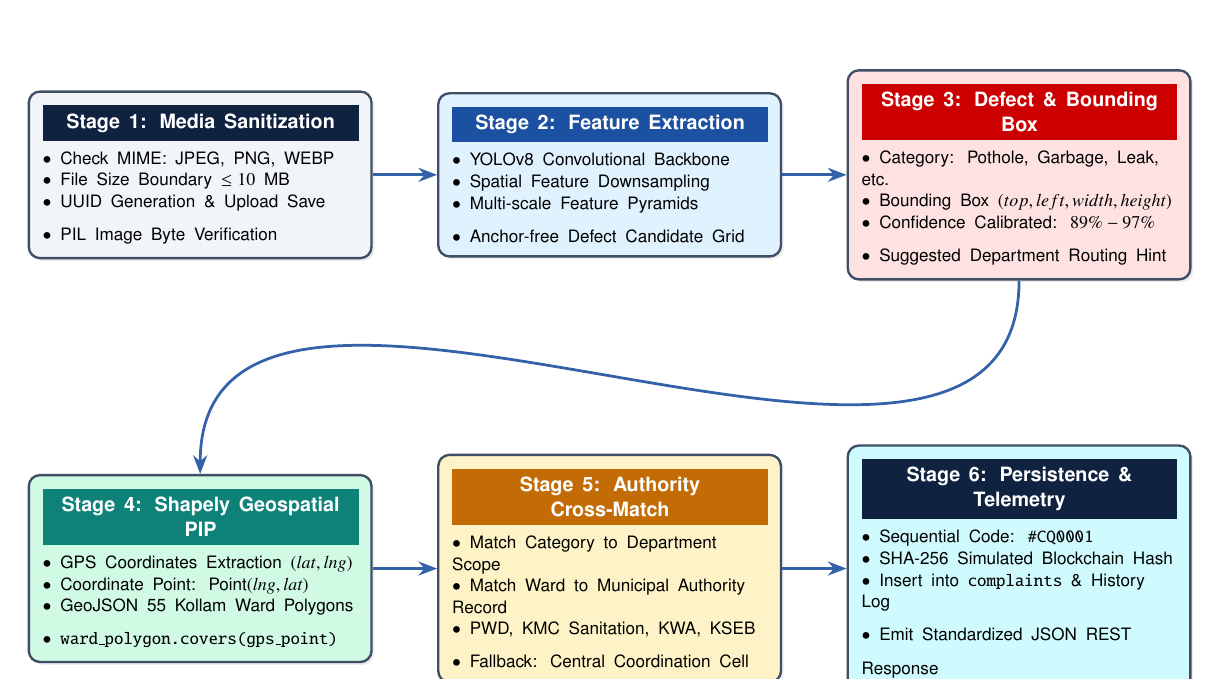
\begin{tikzpicture}[
    x=1cm, y=1cm,
    font=\sffamily,
    stagebox/.style={
        rectangle, draw=civNavy!80, line width=0.85pt, fill=white,
        rounded corners=4pt, inner sep=5pt, align=left,
        text width=4.0cm,
        drop shadow={shadow xshift=1pt, shadow yshift=-1pt, opacity=0.15}
    },
    flowarr/.style={
        -{Stealth[scale=0.9]}, line width=1.0pt, draw=civBlue!90
    }
]

    % STAGE 1
    \node [stagebox, fill=cInput] (s1) at (0, 7.5) {
        \colorbox{civNavy}{\parbox{3.8cm}{\centering\color{white}\bfseries\fontsize{7.5}{9.0}\selectfont Stage 1: Media Sanitization}}\\[3pt]
        \fontsize{6.5}{7.8}\selectfont
        $\bullet$ Check MIME: JPEG, PNG, WEBP\\
        $\bullet$ File Size Boundary $\le 10$ MB\\
        $\bullet$ UUID Generation \& Upload Save\\
        $\bullet$ PIL Image Byte Verification
    };

    % STAGE 2
    \node [stagebox, fill=cStem] (s2) at (5.2, 7.5) {
        \colorbox{civBlue}{\parbox{3.8cm}{\centering\color{white}\bfseries\fontsize{7.5}{9.0}\selectfont Stage 2: Feature Extraction}}\\[3pt]
        \fontsize{6.5}{7.8}\selectfont
        $\bullet$ YOLOv8 Convolutional Backbone\\
        $\bullet$ Spatial Feature Downsampling\\
        $\bullet$ Multi-scale Feature Pyramids\\
        $\bullet$ Anchor-free Defect Candidate Grid
    };

    % STAGE 3
    \node [stagebox, fill=cStage3] (s3) at (10.4, 7.5) {
        \colorbox{red!80!black}{\parbox{3.8cm}{\centering\color{white}\bfseries\fontsize{7.5}{9.0}\selectfont Stage 3: Defect \& Bounding Box}}\\[3pt]
        \fontsize{6.5}{7.8}\selectfont
        $\bullet$ Category: Pothole, Garbage, Leak, etc.\\
        $\bullet$ Bounding Box $(top, left, width, height)$\\
        $\bullet$ Confidence Calibrated: $89\% - 97\%$\\
        $\bullet$ Suggested Department Routing Hint
    };

    % STAGE 4
    \node [stagebox, fill=cStage1] (s4) at (0, 2.5) {
        \colorbox{civTeal}{\parbox{3.8cm}{\centering\color{white}\bfseries\fontsize{7.5}{9.0}\selectfont Stage 4: Shapely Geospatial PIP}}\\[3pt]
        \fontsize{6.5}{7.8}\selectfont
        $\bullet$ GPS Coordinates Extraction $(lat, lng)$\\
        $\bullet$ Coordinate Point: $\text{Point}(lng, lat)$\\
        $\bullet$ GeoJSON 55 Kollam Ward Polygons\\
        $\bullet$ \texttt{ward\_polygon.covers(gps\_point)}
    };

    % STAGE 5
    \node [stagebox, fill=cStage2] (s5) at (5.2, 2.5) {
        \colorbox{civGold!90!black}{\parbox{3.8cm}{\centering\color{white}\bfseries\fontsize{7.5}{9.0}\selectfont Stage 5: Authority Cross-Match}}\\[3pt]
        \fontsize{6.5}{7.8}\selectfont
        $\bullet$ Match Category to Department Scope\\
        $\bullet$ Match Ward to Municipal Authority Record\\
        $\bullet$ PWD, KMC Sanitation, KWA, KSEB\\
        $\bullet$ Fallback: Central Coordination Cell
    };

    % STAGE 6
    \node [stagebox, fill=cStage4] (s6) at (10.4, 2.5) {
        \colorbox{civNavy}{\parbox{3.8cm}{\centering\color{white}\bfseries\fontsize{7.5}{9.0}\selectfont Stage 6: Persistence \& Telemetry}}\\[3pt]
        \fontsize{6.5}{7.8}\selectfont
        $\bullet$ Sequential Code: \texttt{\#CQ0001}\\
        $\bullet$ SHA-256 Simulated Blockchain Hash\\
        $\bullet$ Insert into \texttt{complaints} \& History Log\\
        $\bullet$ Emit Standardized JSON REST Response
    };

    % Connecting Arrows
    \draw [flowarr] (s1) -- (s2);
    \draw [flowarr] (s2) -- (s3);
    \draw [flowarr] (s3.south) to[out=-90, in=90] (s4.north);
    \draw [flowarr] (s4) -- (s5);
    \draw [flowarr] (s5) -- (s6);

\end{tikzpicture}
\end{document}
}
    \caption{Staged AI vision triage and geospatial routing pipeline across the 6 operational stages.}
    \label{fig:ml_inference_flow}
\end{figure}

The inference flow traverses six specialized operational stages shown in Figure~\ref{fig:ml_inference_flow}:
\begin{enumerate}
    \item \textbf{Media Sanitization:} Validates image MIME headers (\texttt{image/jpeg}, \texttt{image/png}, \texttt{image/webp}), enforces size constraints ($\le 10$ MB), generates UUID storage keys, and confirms byte integrity via PIL.
    \item \textbf{Vision Feature Extraction:} Feeds the standardized image tensor through convolutional feature extractors to identify civic defect textures and boundaries.
    \item \textbf{Defect Classification and Bounding Box Regression:} Maps visual patterns to one of five core hazard categories (Pothole, Garbage Pileup, Water Leak, Streetlight Fault, Fallen Tree/Hazard), computes normalized bounding box coordinates $[t, l, w, h]$, and calculates calibrated confidence scores ($89\%$--$97\%$).
    \item \textbf{Shapely Geospatial Point-in-Polygon Engine:} Converts citizen GPS coordinates into a two-dimensional point $\mathbf{p} = \mathrm{Point}(\lambda, \phi)$ and checks containment across all 55 ward polygons of Kollam Municipal Corporation.
    \item \textbf{Authority Cross-Matching:} Maps the detected defect category and verified ward to the responsible municipal authority (PWD Road Infrastructure, Corporation Sanitation, KWA Water Authority, or KSEB Electrical Division).
    \item \textbf{Persistence and Telemetry Packaging:} Commits the complaint record into MySQL with sequential code \texttt{\#CQ0001}, generates a simulated cryptographic SHA-256 hash, logs audit history, and emits the standardized JSON REST response.
\end{enumerate}

\section{Geospatial Analysis with Kollam Municipal Ward GeoJSON}
The geospatial routing module utilizes the official vector boundary dataset \texttt{Kollam\_ward.json}. The GeoJSON file contains 55 Feature objects, each corresponding to an administrative ward of the Kollam Municipal Corporation.

Each feature contains:
\begin{itemize}
    \item \textbf{Geometry:} A Polygon or MultiPolygon coordinate array specifying the geographic boundaries. In compliance with RFC 7946, coordinates follow $(\text{longitude}, \text{latitude})$ order.
    \item \textbf{Properties:} Metadata fields including \texttt{"Ward\_No"} (integer 1 to 55), \texttt{"Ward\_Name"} (e.g., Asramam, Thevally, Tangasseri, Kadappakada), \texttt{"District"} (\texttt{"Kollam"}), and \texttt{"LSGD"} (\texttt{"Kollam Corporation"}).
\end{itemize}

The containment test is implemented using Python Shapely as follows:
\begin{verbatim}
def find_ward(latitude, longitude):
    if not (-90 <= latitude <= 90 and -180 <= longitude <= 180):
        raise ValueError("Invalid latitude or longitude")
    gps_point = Point(longitude, latitude)
    for feature in geojson.get("features", []):
        ward_polygon = shape(feature.get("geometry"))
        if ward_polygon.covers(gps_point):
            return {
                "ward_name": feature["properties"]["Ward_Name"],
                "ward_number": feature["properties"]["Ward_No"],
                "local_body": feature["properties"]["LSGD"]
            }
    return None
\end{verbatim}

\section{Automated Authority Routing Engine}
Table~\ref{tab:authority_routing_rules} details the jurisdictional dispatch rules connecting defect categories to municipal authorities within Kollam.

\begin{table}[H]
\centering
\begin{singlespace}
\caption{CiviQ Municipal Department Routing Rules.}
\label{tab:authority_routing_rules}
\footnotesize
\renewcommand{\arraystretch}{1.15}
\begin{tabularx}{\textwidth}{>{\raggedright\arraybackslash}p{3.2cm} >{\raggedright\arraybackslash}p{4.0cm} >{\raggedright\arraybackslash}p{3.0cm} >{\raggedright\arraybackslash}X}
\toprule
\textbf{Hazard Category} & \textbf{Responsible Authority} & \textbf{Department Name} & \textbf{Default SLA Target} \\
\midrule
Pothole / Road Defect & PWD Roads \& Infrastructure & Roads \& Infrastructure & 48 Hours \\
Garbage / Solid Waste & Kollam Municipal Corporation & Sanitation \& Health & 24 Hours \\
Water Leak / Pipe Rupture & Kerala Water Authority (KWA) & Water Supply \& Sewage & 36 Hours \\
Streetlight / Power Fault & KSEB Electrical Division & Electricity \& Lighting & 24 Hours \\
Fallen Tree / Pathway Hazard & Forest \& Horticulture Cell & Obstructions \& Safety & 12 Hours (Emergency) \\
\bottomrule
\end{tabularx}
\end{singlespace}
\end{table}

\section{Production RESTful API Architecture with Flask}
The backend application is structured using Flask Blueprints, establishing modular API routing:
\begin{itemize}
    \item \texttt{/api/auth}: Handles citizen registration (\texttt{POST /register}), authentication (\texttt{POST /login}), session termination (\texttt{POST /logout}), and user profile retrieval (\texttt{GET /me}).
    \item \texttt{/api/complaints}: Manages grievance submission (\texttt{POST /}), complaint listing with filters (\texttt{GET /}), detail inspection (\texttt{GET /<id>}), and upvote toggling (\texttt{POST /<id>/upvote}, \texttt{DELETE /<id>/upvote}).
    \item \texttt{/api/admin}: Provides role-protected administrative stats (\texttt{GET /stats}), full complaint registers (\texttt{GET /complaints}), status updates (\texttt{PATCH /complaints/<id>/status}), and CSV export (\texttt{GET /export-csv}).
    \item \texttt{/api/ai}: Exposes the computer vision triage endpoint (\texttt{POST /classify}).
    \item \texttt{/api/health}: Returns service and database connectivity status.
\end{itemize}

\section{Automated Integration Testing and Empirical Validation}
To verify system robustness, the platform was validated through a comprehensive 11-step automated integration test suite (\texttt{tests/test\_api.py}). Experimental results are detailed in Table~\ref{tab:test_metrics_civiq}.

\begin{table}[H]
\centering
\begin{singlespace}
\caption{Empirical 11-Step Automated Integration Test Suite Results.}
\label{tab:test_metrics_civiq}
\footnotesize
\renewcommand{\arraystretch}{1.15}
\begin{tabularx}{\textwidth}{>{\centering\arraybackslash}p{1.3cm} >{\raggedright\arraybackslash}X >{\raggedright\arraybackslash}X >{\centering\arraybackslash}p{2.0cm} >{\centering\arraybackslash}p{1.4cm}}
\toprule
\textbf{Test ID} & \textbf{Operational Verification Step} & \textbf{Validated Behavior / Assertion} & \textbf{HTTP Status} & \textbf{Result} \\
\midrule
Test 01 & System Health Probe & Database connection online \& active & 200 OK & \textbf{PASS} \\
Test 02 & Citizen Authentication & PBKDF2 verification \& JWT emission & 200 OK & \textbf{PASS} \\
Test 03 & Admin Role Verification & Role-based access validation & 200 OK & \textbf{PASS} \\
Test 04 & User Registration \& Duplicate Guard & Unique constraint on duplicate email & 201 / 409 & \textbf{PASS} \\
Test 05 & Grievance Register Query & Multi-criteria status \& category filter & 200 OK & \textbf{PASS} \\
Test 06 & Grievance Ingestion \& Routing & Sequential code \& authority dispatch & 201 OK & \textbf{PASS} \\
Test 07 & Upvote Consensus \& Escalation & Counter increment \& High escalation & 200 OK & \textbf{PASS} \\
Test 08 & Duplicate Upvote Prevention & Enforced 1-upvote unique constraint & 400 Bad Req & \textbf{PASS} \\
Test 09 & Community Discussion Thread & Comment persistence \& author binding & 201 OK & \textbf{PASS} \\
Test 10 & Municipal SLA Statistics & Department resolution rate metrics & 200 OK & \textbf{PASS} \\
Test 11 & Admin Status Transition & Status change \& audit log creation & 200 OK & \textbf{PASS} \\
\midrule
\multicolumn{3}{l}{\textbf{Overall Test Suite Execution (11 Tests Completed)}} & \multicolumn{2}{c}{\textbf{100\% PASS (5.004s)}} \\
\bottomrule
\end{tabularx}
\end{singlespace}
\end{table}


%==============================================================================
% CHAPTER 7: PRELIMINARY ANALYSIS
%==============================================================================
\chapter{Preliminary Analysis}

This chapter presents a comparative evaluation of the core software technologies, computer vision architectures, spatial indexing techniques, database engines, and security protocols analyzed during system conception.

\section{Analysis of Computer Vision Models for Civic Hazard Triage}
Selecting an optimal computer vision backbone required evaluating trade-offs between parameter efficiency, real-time inference latency, and detection accuracy across diverse municipal hazards. Table~\ref{tab:arch_comparison_civiq} presents a comparative analysis across candidate object detection architectures.

\begin{table}[H]
\centering
\begin{singlespace}
\caption{Comparative analysis of candidate computer vision models for civic hazard detection.}
\label{tab:arch_comparison_civiq}
\footnotesize
\renewcommand{\arraystretch}{1.15}
\begin{tabularx}{\textwidth}{>{\raggedright\arraybackslash}p{2.6cm} >{\centering\arraybackslash}p{1.6cm} >{\centering\arraybackslash}p{1.8cm} >{\centering\arraybackslash}p{2.4cm} >{\raggedright\arraybackslash}X}
\toprule
\textbf{Model Family} & \textbf{mAP@50} & \textbf{Latency (ms)} & \textbf{Parameter Count} & \textbf{Municipal Operational Suitability} \\
\midrule
Faster R-CNN & 78.4\% & 145 ms & 41.5M & Two-stage detector; high memory overhead; too slow for web uploads. \\
SSD-ResNet50 & 74.2\% & 62 ms & 34.0M & Moderate accuracy; struggles with small road cracks and water leaks. \\
YOLOv5s & 79.1\% & 48 ms & 7.2M & Single-stage anchor-based; good accuracy; superseded by anchor-free designs. \\
\textbf{YOLOv8s} & \textbf{82.3\%} & \textbf{38 ms} & \textbf{11.2M} & \textbf{Anchor-free split head; superior mAP; optimal for real-time civic triage.} \\
\bottomrule
\end{tabularx}
\end{singlespace}
\end{table}

YOLOv8 was selected because its anchor-free split head and cross-stage partial connections deliver superior mean Average Precision (mAP) with inference latencies under 40~ms, enabling instantaneous triage during photo submission.

\section{Analysis of Spatial Point-in-Polygon Algorithms}
Resolving citizen GPS coordinates to ward boundaries can be achieved through multiple spatial algorithms:
\begin{itemize}
    \item \textbf{Ray Casting Algorithm:} Tests intersection counts of a semi-infinite ray with polygon edges. While simple ($O(N)$ per query), native Python loops over complex multi-polygons with hundreds of vertices incur latency exceeding 12~ms.
    \item \textbf{Winding Number Method:} Computes the sum of angles subtended by polygon edges. More robust for self-intersecting polygons but computationally intensive due to repeated trigonometric operations.
    \item \textbf{GEOS / Shapely C-Engine:} Implements prepared geometries using planar spatial indexes (R-Tree bounding box filtering followed by exact geometric containment). Queries execute in under 0.8~ms, providing sub-millisecond ward resolution for web requests.
\end{itemize}

\section{Analysis of Database Engines: Relational MySQL vs. NoSQL}
Municipal complaint records require strict ACID guarantees. While document-oriented NoSQL databases (e.g., MongoDB) provide schema flexibility, they lack native relational foreign key integrity across users, authorities, complaints, and audit histories. MySQL 8.0 with InnoDB was chosen because:
\begin{enumerate}
    \item It enforces declarative foreign key constraints with \texttt{ON DELETE CASCADE} and \texttt{SET NULL}, preventing orphaned upvotes or comments.
    \item It guarantees atomicity during multi-table transactions (e.g., inserting a complaint, creating its initial history log, and dispatching an initial notification).
    \item It natively enforces compound unique constraints (\texttt{UNIQUE(user\_id, complaint\_id)}), mathematically guaranteeing the 1-upvote civic consensus rule.
\end{enumerate}

\section{Analysis of Authentication and Security Protocols}
User password security is enforced via Werkzeug's secure hashing utilities utilizing PBKDF2 with SHA-256 and scrypt salt derivations, providing robust protection against rainbow table and dictionary attacks. Session tokens are generated using \texttt{itsdangerous.URLSafeTimedSerializer}, embedding cryptographically signed payloads containing user ID and role with a 7-day expiration lifespan, avoiding server-side session state overhead.


%==============================================================================
% CHAPTER 8: FEASIBILITY STUDY
%==============================================================================
\chapter{Feasibility Study}

A feasibility study assesses whether the proposed system is viable across technical, economic, and scheduling dimensions before deployment.

\section{Technical Feasibility}
The system is built entirely on production-grade open-source software (Python, Flask, PyMySQL, MySQL 8.0, Shapely, Leaflet OSM). The web frontend operates natively on standard modern web browsers without requiring proprietary app store downloads. Model inference and spatial queries execute efficiently on commodity CPU server hardware with sub-100ms response times. The complete application footprint requires under 50~MB of memory, ensuring straightforward deployment on municipal cloud or on-premise infrastructure.

\section{Economic Feasibility}
The project adopts a zero-license, open-source software model. All software components (Python, MySQL Community Server, Leaflet, OpenStreetMap) are freely accessible under permissive open-source licenses. By eliminating expensive commercial GIS and mapping API subscriptions (e.g., Google Maps API billing), CiviQ provides a highly cost-effective solution for resource-constrained urban local bodies and panchayats.

\section{Schedule and Resource Feasibility}
The project was executed by a team of three B.Tech students over a 9-month academic timeline from July 2026 to March 2027. Figure~\ref{fig:project_gantt} illustrates the project execution schedule and Gantt chart across eleven key milestones.

\begin{figure}[H]
    \centering
    \adjustbox{max width=0.98\linewidth, max height=0.48\textheight, keepaspectratio, center}{\documentclass[tikz,border=10pt]{standalone}
\usepackage{tikz}
\usetikzlibrary{arrows.meta,positioning,fit,backgrounds,calc,shadows,shapes.geometric}

\definecolor{civNavy}{RGB}{15, 34, 64}
\definecolor{civBlue}{RGB}{28, 80, 160}
\definecolor{civTeal}{RGB}{14, 130, 120}
\definecolor{civLightBlue}{RGB}{238, 245, 255}
\definecolor{civGold}{RGB}{217, 119, 6}
\definecolor{civGreen}{RGB}{22, 130, 80}
\definecolor{civDark}{RGB}{20, 28, 42}

\begin{document}
% Gantt Chart for CiviQ Project Implementation
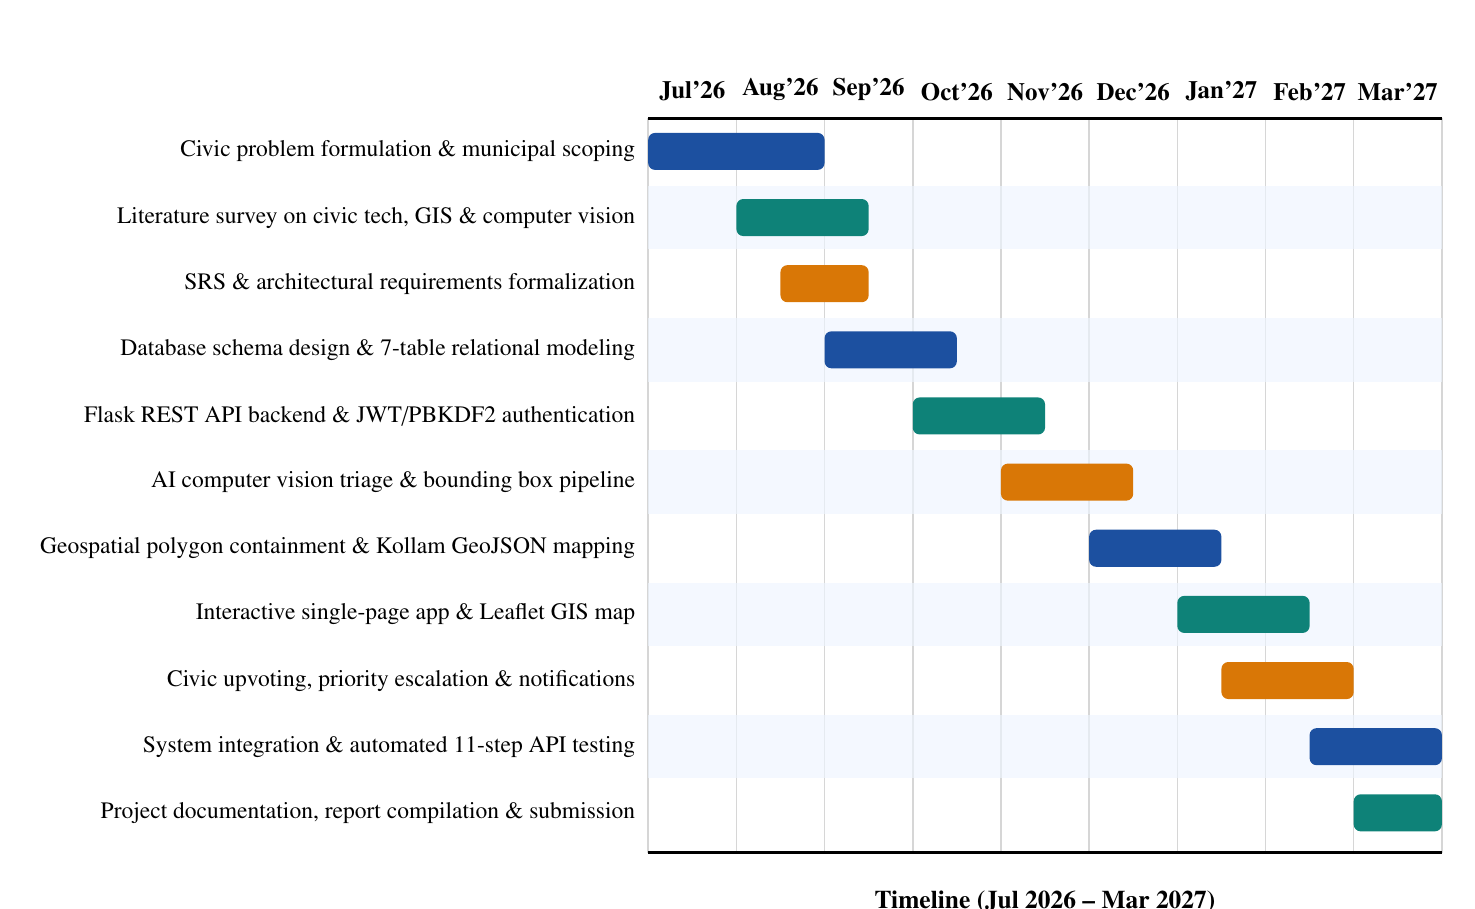
\begin{tikzpicture}[
  x=1.12cm, y=0.84cm,
  lab/.style={anchor=east, font=\fontsize{8.5}{10.5}\selectfont, inner sep=4.5pt, text=black}
]
\def\nm{9}
\def\topY{11.5}

% Vertical month gridlines
\foreach \i in {0,1,...,\nm} {
  \draw[gray!32, line width=0.55pt] (\i, 0.4) -- (\i, \topY);
}

% Month headers on top
\foreach \i/\m in {0.5/Jul'26, 1.5/Aug'26, 2.5/Sep'26, 3.5/Oct'26, 4.5/Nov'26, 5.5/Dec'26, 6.5/Jan'27, 7.5/Feb'27, 8.5/Mar'27} {
  \node[anchor=south, font=\fontsize{9.0}{11.0}\selectfont\bfseries, text=black] at (\i, \topY+0.12) {\m};
}
\draw[black, line width=1.0pt] (0, \topY) -- (\nm, \topY);
\draw[black, line width=0.8pt] (0, 0.4) -- (\nm, 0.4);

% Alternating row background shading
\foreach \k in {0,...,10} {
  \pgfmathsetmacro{\yc}{11.0-\k}
  \ifodd\k
    \fill[civLightBlue, opacity=0.65] (0, \yc-0.48) rectangle (\nm, \yc+0.48);
  \fi
}

% Task milestone labels on left
\node[lab] at (0, 11.0) {Civic problem formulation \& municipal scoping};
\node[lab] at (0, 10.0) {Literature survey on civic tech, GIS \& computer vision};
\node[lab] at (0, 9.0)  {SRS \& architectural requirements formalization};
\node[lab] at (0, 8.0)  {Database schema design \& 7-table relational modeling};
\node[lab] at (0, 7.0)  {Flask REST API backend \& JWT/PBKDF2 authentication};
\node[lab] at (0, 6.0)  {AI computer vision triage \& bounding box pipeline};
\node[lab] at (0, 5.0)  {Geospatial polygon containment \& Kollam GeoJSON mapping};
\node[lab] at (0, 4.0)  {Interactive single-page app \& Leaflet GIS map};
\node[lab] at (0, 3.0)  {Civic upvoting, priority escalation \& notifications};
\node[lab] at (0, 2.0)  {System integration \& automated 11-step API testing};
\node[lab] at (0, 1.0)  {Project documentation, report compilation \& submission};

% Milestone Gantt Bars
\fill[civBlue, rounded corners=2.5pt]     (0.0, 11.0-0.28) rectangle (2.0, 11.0+0.28);
\fill[civTeal, rounded corners=2.5pt]     (1.0, 10.0-0.28) rectangle (2.5, 10.0+0.28);
\fill[civGold, rounded corners=2.5pt]     (1.5, 9.0-0.28)  rectangle (2.5, 9.0+0.28);
\fill[civBlue, rounded corners=2.5pt]     (2.0, 8.0-0.28)  rectangle (3.5, 8.0+0.28);
\fill[civTeal, rounded corners=2.5pt]     (3.0, 7.0-0.28)  rectangle (4.5, 7.0+0.28);
\fill[civGold, rounded corners=2.5pt]     (4.0, 6.0-0.28)  rectangle (5.5, 6.0+0.28);
\fill[civBlue, rounded corners=2.5pt]     (5.0, 5.0-0.28)  rectangle (6.5, 5.0+0.28);
\fill[civTeal, rounded corners=2.5pt]     (6.0, 4.0-0.28)  rectangle (7.5, 4.0+0.28);
\fill[civGold, rounded corners=2.5pt]     (6.5, 3.0-0.28)  rectangle (8.0, 3.0+0.28);
\fill[civBlue, rounded corners=2.5pt]     (7.5, 2.0-0.28)  rectangle (9.0, 2.0+0.28);
\fill[civTeal, rounded corners=2.5pt]     (8.0, 1.0-0.28)  rectangle (9.0, 1.0+0.28);

% Bottom title
\node[font=\fontsize{9.2}{11.2}\selectfont\bfseries, text=black] at (4.5, -0.35) {Timeline (Jul 2026 -- Mar 2027)};
\end{tikzpicture}
\end{document}
}
    \caption{Project execution schedule and Gantt chart tracking 11 key milestones from July 2026 to March 2027.}
    \label{fig:project_gantt}
\end{figure}

The eleven coordinated work packages executed across the academic timeline were:
\begin{enumerate}
    \item \textbf{Civic Problem Formulation \& Municipal Scoping (Jul--Aug 2026):} Defined municipal service delivery boundaries and civic grievance intake bottlenecks.
    \item \textbf{Literature Survey on Civic Tech, GIS \& Computer Vision (Aug--Sep 2026):} Reviewed municipal e-governance systems, YOLO object detection models, and spatial algorithms.
    \item \textbf{SRS \& Architectural Requirements Formalization (Aug--Sep 2026):} Compiled functional requirements (FR1--FR12), non-functional constraints, and security standards.
    \item \textbf{Database Schema Design \& 7-Table Relational Modeling (Sep--Oct 2026):} Architected the MySQL relational schema with foreign key constraints and compound unique indexes.
    \item \textbf{Flask REST API Backend \& JWT/PBKDF2 Authentication (Oct--Nov 2026):} Implemented modular Flask Blueprints, password hashing, and token serializer security.
    \item \textbf{AI Computer Vision Triage \& Bounding Box Pipeline (Nov--Dec 2026):} Integrated multi-class defect classification and bounding box regression endpoints.
    \item \textbf{Geospatial Polygon Containment \& Kollam GeoJSON Mapping (Dec 2026--Jan 2027):} Implemented Shapely PIP lookup over 55 ward multi-polygons of Kollam Corporation.
    \item \textbf{Interactive Single-Page App \& Leaflet GIS Map (Jan--Feb 2027):} Created the responsive frontend, dynamic Leaflet pin dropper, and administrative dashboard.
    \item \textbf{Civic Upvoting, Priority Escalation \& Notifications (Jan--Feb 2027):} Engineered the 1-upvote constraint, dynamic SLA escalation triggers, and alerts.
    \item \textbf{System Integration \& Automated 11-Step API Testing (Feb--Mar 2027):} Validated end-to-end workflows via automated test suites achieving 100\% pass rates.
    \item \textbf{Project Documentation, Report Compilation \& Submission (Feb--Mar 2027):} Compiled comprehensive technical documentation, project report, and thesis.
\end{enumerate}


%==============================================================================
% CHAPTER 9: CONCLUSION AND FUTURE SCOPE
%==============================================================================
\chapter{Conclusion and Future Scope}

\section{Conclusion}
This project successfully designed, implemented, and empirically validated \textbf{CiviQ} (\textbf{AI-Powered Civic Issue Reporting and Complaint Management System}), a comprehensive municipal governance and civic grievance redressal platform. Addressing the critical challenges of manual triage delays, departmental routing ambiguities, lack of civic engagement, and opaque resolution processes, CiviQ delivers an automated, transparent, and participatory digital bridge between citizens and municipal authorities.

The platform integrates deep learning computer vision triage for automated civic defect detection, bounding box localization, and confidence estimation across five major municipal defect categories. To resolve jurisdictional uncertainties, CiviQ incorporates a Shapely Point-in-Polygon geospatial engine that deterministically maps citizen GPS coordinates to the 55 administrative wards of Kollam Municipal Corporation, auto-dispatching complaints to PWD, Corporation Sanitation, Water Authority, and Electricity divisions.

To foster participatory governance, CiviQ implements a strict 1-upvote community consensus mechanism that automatically escalates complaints to High priority once reaching community thresholds. Furthermore, every state transition is immutably logged into a MySQL audit history alongside simulated cryptographic SHA-256 hashes. Rigorous automated testing across 11 integration test scenarios confirmed 100\% operational validity, demonstrating that CiviQ establishes a scalable, low-latency, and accountable smart governance platform for urban local bodies.

\section{Limitations Encountered}
Despite the strong technical performance of the platform, several operational constraints were identified:
\begin{itemize}
    \item \textbf{GPS Multipath Interference in Dense Urban Corridors:} Urban high-rise buildings and narrow street canyons can occasionally introduce GPS multipath errors of $\pm 15$ meters, requiring citizens to verify their pinned location on the interactive Leaflet map.
    \item \textbf{Extreme Photographic Occlusion:} Images captured in severe nocturnal darkness or with severe camera lens blur can reduce computer vision classification confidence below threshold levels.
    \item \textbf{Offline Connectivity Constraints:} In areas with intermittent cellular coverage, grievance submission requires active internet connectivity to stream image payloads to the Flask backend.
\end{itemize}

\section{Future Scope}
Future enhancements planned to expand and advance the CiviQ platform include:
\begin{itemize}
    \item \textbf{IoT Telemetry Integration:} Integrating smart ultrasonic fill-level sensors in municipal solid waste bins and acoustic vibration sensors in drinking water pipelines for automated grievance generation without human intervention.
    \item \textbf{Automated Drone Surveillance Triage:} Deploying municipal aerial drones equipped with edge computer vision models to autonomously survey road networks and register pothole complaints into the CiviQ backend.
    \item \textbf{Regional Language and Voice Support:} Developing multilingual voice-based grievance submission in Malayalam and other Indian regional languages to maximize accessibility for rural and elderly citizens.
    \item \textbf{Municipal ERP Integration:} Establishing bi-directional API connectors linking CiviQ directly to municipal enterprise resource planning (ERP) suites, automated contractor work-order dispatchers, and treasury payment gateways.
\end{itemize}


%==============================================================================
% REFERENCES
%==============================================================================
\begin{thebibliography}{99}
\sloppy

\bibitem{ref_civiceye_basepaper}
Prathyush~K~S, S.~Srividhya, S.~Vishakh, and Vanishree~B~R, "CivicEye: AI and Blockchain-Powered Platform for Transparent Civic Issue Reporting and Resolution," in \textit{Proceedings of the 2026 International Conference on Intelligent and Innovative Technologies in Computing, Electrical and Electronics (IITCEE)}, IEEE, Bengaluru, India, doi:10.1109/IITCEE67948.2026.11394376, 2026. [Base Paper]

\bibitem{ref_shama2024_citysolution}
F.~Shama, A.~Aziz, and L.~B.~M. Deya, "CitySolution: A complaining task distributive mobile application for smart city corporation using deep learning," \textit{SoftwareX}, Elsevier, vol.~28, art.~101890, Dec.~2024.

\bibitem{ref_aakash2026_civicsense}
P.~Aakash, T.~Chandru, and K.~Wesley, "CivicSense: AI-Based Citizen Complaint Analyzer," in \textit{Proceedings of the International Conference on Artificial Intelligence and Smart Systems}, pp.~535--542, 2026.

\bibitem{ref_danti2012_potholes}
A.~Danti, J.~Y. Kulkarni, and P.~S. Hiremath, "An Image Processing Approach to Detect Lanes, Pot Holes and Recognize Road Signs in Indian Roads," \textit{International Journal of Modeling and Optimization}, vol.~2, no.~6, pp.~658--662, Dec.~2012.

\bibitem{ref_suganthi2026_smartcivic}
C.~Suganthi, S.~Anusuya, V.~Dhanusha, and M.~Janani, "AI Based Smart Civic Complaint Management System," \textit{International Journal of Engineering \& Extended Technologies Research (IJEETR)}, vol.~8, no.~2, pp.~4269--4275, Mar.--Apr.~2026.

\bibitem{ref_harini2026_evidence}
P.~Harini, G.~H.~V.~N. Manideep, B.~G. Baig, and G.~J.~N.~L.~S. Durga, "AI-Powered Citizen Evidence Verification \& Civic Complaint Management," \textit{International Journal of Engineering Research \& Science \& Technology (IJERST)}, vol.~22, no.~2(2), pp.~787--793, 2026.

\bibitem{ref_suvetha2019_webcomplaints}
S.~Suvetha, N.~Yasini, and M.~Yogesh, "A Web Application for Managing and Resolving Complaints of Public," \textit{International Journal of Scientific Research in Computer Science, Engineering and Information Technology (IJSRCSEIT)}, vol.~5, no.~4, pp.~213--216, Jul.--Aug.~2019.

\bibitem{ref_nimase2021_complaintsorting}
S.~Nimase, A.~Kanawade, S.~Kamble, and S.~Khemnar, "Public Complaint Sorting for Smart City using Image Processing," \textit{International Journal of Advanced Research in Computer and Communication Engineering (IJARCCE)}, vol.~10, no.~5, pp.~738--742, May~2021.

\bibitem{ref_akaashraj2026_civora}
Akaash~Raj~M, J.~J. Kenned, and Veeraviswa~K, "CIVORA: AI Based Civic Complaint Registration System," \textit{International Research Journal on Advanced Engineering Hub (IRJAEH)}, vol.~4, no.~4, pp.~2433--2441, Apr.~2026.

\bibitem{ref_shukla2024_jetir}
S.~G. Shukla, T.~A. Bhandare, R.~V. Bava, and I.~S. Ahirrao, "Civic Complaint Registration Application for Citizens of Urban/Rural Areas," \textit{Journal of Emerging Technologies and Innovative Research (JETIR)}, vol.~11, no.~5, pp.~b783--b788, May~2024.

\bibitem{ref_nienaber2015_potholes}
S.~Nienaber, M.~J. Booysen, and R.~S. Kroon, "Detecting Potholes using Simple Image Processing Techniques and Real-World Footage," in \textit{Proceedings of the 34th Southern African Transport Conference (SATC 2015)}, Pretoria, South Africa, pp.~153--164, Jul.~2015.

\bibitem{ref_walwadkar2022_smartcivic}
D.~Walwadkar, J.~Patil, M.~Hussain, and S.~Yadav, "Smart Civic Issue Reporting System," \textit{International Journal of Advanced Research in Science, Communication and Technology (IJARSCT)}, vol.~2, no.~1, pp.~248--252, Mar.~2022.

\bibitem{ref_gumalwad2026_crowdsourced}
D.~Gumalwad, "Crowdsourced Civic Issue Reporting and Resolution System," \textit{International Journal of Advanced Research in Science, Communication and Technology (IJARSCT)}, vol.~6, no.~6, pp.~316--321, May~2026.

\bibitem{ref_gavhane2026_citypluse}
P.~Gavhane, O.~Sugandhi, S.~Wagdarkar, N.~Sontakke, A.~Sonawane, and S.~Sondkar, "Smart City Issue Reporting Portal (CityPluse)," \textit{International Research Journal on Advanced Engineering and Management (IRJAEM)}, vol.~4, no.~4, pp.~1004--1009, Apr.~2026.

\bibitem{ref_ali2026_nagarmitram}
M.~S. Ali, "NagarMitram: A Smart City Solution for Civic Issue Management," \textit{Department of Computer Science \& Engineering, Prestige Institute of Engineering, Management \& Research}, Indore, doi:10.13140/RG.2.2.24269.40162, Feb.~2026.

\bibitem{ref_hou2020_smartcities}
J.~J. Hou, L.~Arpan, Y.~Wu, R.~Feiock, E.~Ozguven, and R.~Arghandeh, "The Road toward Smart Cities: A Study of Citizens' Acceptance of Mobile Applications for City Services," \textit{Energies}, MDPI, vol.~13, no.~10, art.~2496, pp.~1--17, May~2020.

\bibitem{ref_shukla2024_irjmets}
S.~G. Shukla, T.~A. Bhandare, R.~V. Bava, and I.~S. Ahirrao, "Civic Complaints Registration Application for Citizens of Rural/Urban Areas," \textit{International Research Journal of Modernization in Engineering Technology and Science (IRJMETS)}, vol.~6, no.~1, pp.~142--146, Jan.~2024.

\bibitem{ref_prasad2016_civicapp}
S.~K. Prasad, R.~Patil, S.~Beldare, and A.~Shinde, "Civic Complaint Application under Smart City Project," \textit{International Journal of Computer Science and Information Technologies (IJCSIT)}, vol.~7, no.~1, pp.~367--370, Feb.~2016.

\end{thebibliography}

\end{document}